% !Mode:: "Tex:UTF-8"


El contraste de hipótesis es, junto con la estimación mediante intervalos de confianza, el otro gran ingrediente de la Inferencia Estadística clásica. En el Capítulo \ref{cap:IntervalosConfianza} hemos aprendido a construir intervalos de confianza para la media y la varianza. En este capítulo vamos a estudiar la técnica del contraste de hipótesis, centrándonos en ese mismo problema de la media. Y una vez que hayamos entendido el esquema básico de ambas técnicas, en los próximos capítulos vamos a extenderlas, en paralelo, a otras situaciones, de manera que podemos decir que, por cada nuevo intervalo de confianza que aprendamos a calcular, habrá un contraste de hipótesis asociado.

\noindent{\bf Advertencia:} En este capítulo, como no hay riesgo de confusión, vamos a escribir $\mu$ en lugar de $\mu_X$.

\section{El lenguaje del contraste de hipótesis.}
\label{cap07:sec:LenguajeContrasteHipotesis}

\subsection{Un esquema básico para el método científico.}
\label{cap07:subsec:EsquemaBasicoMetodoCientifico}

El lenguaje del contraste de hipótesis es un ingrediente fundamental del método científico, hasta el punto de que, en las revistas científicas, no se concibe una publicación sobre resultados observacionales, o experimentales, que no utilice este lenguaje. ¿Cómo funciona, en este sentido, el método científico? Vamos a hacer una descripción bastante esquemática, pero que nos va a servir de introducción a la discusión de este capítulo.

    \begin{enumerate}
        \item Un científico propone una \index{hipótesis}{\sf hipótesis}. Es decir, una afirmación, que debe ser susceptible de ser comprobada o negada mediante hechos. No queremos, ni podemos, entrar en una discusión profunda sobre epistemología. Pero eso no significa que esa discusión no sea importante. De hecho, creemos que es esencial para cualquiera que utilice en su trabajo el método científico. En el Apéndice \ref{apendice:comentarioBibliografia}, {\em Bibliografía Comentada}, recomendaremos algunas lecturas, que creemos que pueden ayudar al lector en ese sentido. Aquí nos limitamos a subrayar que, para que una afirmación se pueda considerar una hipótesis susceptible de ser examinada mediante el método científico, tiene que venir acompañada de un procedimiento que permita, utilizando datos, demostrar que esa hipótesis es {\em falsa}. Aunque a menudo se dice que la Ciencia es la búsqueda de la ``Verdad'', en el método científico no nos preocupa demostrar que algo es cierto; eso no forma parte del trabajo de un científico. Lo que se busca es un método lo más eficaz posible para detectar lo que es falso. Entendiendo por falsas las afirmaciones que son incompatibles con los datos de los que disponemos.

        \item Esa afirmación debe probarse mediante la obtención de una colección de datos, una {\em muestra}\index{muestra} o serie de muestras, en el lenguaje que venimos utilizando en el curso. Un ejemplo clásico de recolección de datos es el {\em experimento}, en condiciones controladas y con un alto grado de reproducibilidad. Pero debe quedar claro que el experimento no es la única forma de obtener datos. Los estudios observacionales (como los estudios de campo), las encuestas, la Minería de Datos, etc., también permiten obtener datos relacionados con una hipótesis.  A pesar de eso, en general hablamos de Diseño Experimental para referirnos a las técnicas de recolección de datos. En esta fase, es crucial que el diseño del experimento sea correcto. De nuevo, no podemos entrar a fondo en el tema del Diseño Experimental, y nos remitimos al Apéndice \ref{apendice:MasAlla} del curso, en el que trataremos de ofrecer al lector varias opciones y referencias para avanzar en esta dirección.

        \item Con los datos a nuestra disposición, comienza la fase de \index{análisis estadístico}{\sf análisis estadístico de los datos}. Esta es la fase en la que nos vamos a concentrar en este capítulo. Nuestro objetivo es estudiar la forma en que podemos usar la Estadística para someter a escrutinio una hipótesis, usando los datos de los que disponemos. De nuevo, veremos como la Teoría de la Probabilidad es la herramienta clave en este paso.
    \end{enumerate}

Para ilustrar este esquema, e introducir la terminología necesaria, usaremos un largo ejemplo (dejamos al lector la tarea de decidir si es ficticio).

\begin{ejemplo}\label{cap07:ejem:CangurosDepresivos01}
    Hemos desarrollado un nuevo fármaco, {\em Pildorín Complex}, para tratar la depresión severa en el {\em Canguro Rojo}\index{canguro rojo} australiano\marginpar{\hspace{1.5cm}\includegraphics*[scale=1,width=1cm,keepaspectratio=true]{../fig/Cap07-Canguro2-bn.png}}
    (más información en el enlace [\,\ref{enlace0015}\,]\label{enlace0015a}
    ). Y sostenemos que el medicamento es tan bueno que,  después de administrárselo, los pacientes darán saltos de alegría. De hecho, afirmamos que ``la altura de esos saltos será mucho mayor de lo que era, antes del tratamiento''.

    Para obtener datos relacionados con nuestra afirmación, hemos seleccionado cuidadosamente un grupo de cien canguros depresivos, a los que administramos el medicamento. Medimos con precisión la altura de sus saltos, antes y después de tratarlos. Y nos ponemos muy contentos, porque la altura media de sus saltos, después de usar {\em Pildorín}, es mayor.

    Pero el laboratorio de la competencia, que lleva años vendiendo su medicamento {\em Saltaplus Forte}, replica enseguida que nuestro medicamento no tiene efectos, y que los saltos que hemos observado en nuestros canguros depresivos son, simplemente, sus saltos habituales, que los canguros a veces saltan más y a veces menos, y que nuestras medidas son simplemente {\sf fruto del  azar}.

    La última frase es esencial, porque abre claramente la puerta por la que la Teoría de la Probabilidad entra en esta discusión, para mediar entre nuestra hipótesis y las afirmaciones de la competencia. Porque es verdad que los canguros ya daban saltos, aleatoriamente más o menos altos, antes de tomar nuestro medicamento. ¿Podemos usar la Estadística y la Probabilidad, para demostrar que el uso de {\em {\em Pildorín Complex}} ha tenido realmente un {\em efecto} sobre la altura de los saltos de los canguros depresivos? Bueno, naturalmente, para empezar a definir lo que consideramos un {\em efecto}, necesitamos saber algo sobre la altura típica de los saltos de los canguros depresivos sin medicar. Así que le preguntamos a un experto independiente, ¿cuánto saltan los canguros depresivos (insistimos, sin medicar)? Vamos a suponer que el experto nos dice que la altura (en metros) de los saltos se puede representar mediante una variable aleatoria, que sigue una distribución normal, con media $\mu_0=2.5$ (en metros). Nosotros hemos observado en nuestra muestra de 100 canguros depresivos tratados con {\em {\em Pildorín Complex}} una altura de salto media $\bar X=2.65$ (en metros), con desviación típica muestral $s=0.5$. Esto podría ser fruto del azar, claro está. Pero la pregunta clave es ¿cómo de sorprendente, cómo de rara, excepcional e inexplicable le parece esa muestra al experto? Normalmente este tipo de situaciones quedan más claras si exageramos el efecto del medicamento: si, después de darles el tratamiento, los canguros dieran saltos de 10m en promedio, al experto (y a la competencia) le costaría mucho decir ``bueno, será cosa del azar''.\qed
\end{ejemplo}
Como hemos dicho al final de este ejemplo, el objetivo de un contraste de hipótesis consiste, hablando informalmente, en establecer cómo de sorprendentes,  inesperados o inexplicables le parecen los resultados de la muestra a alguien {\em que no acepta, o no se cree, nuestra hipótesis de trabajo}. Así pues, para empezar a entender la mecánica del contraste de hipótesis, nos servirá de ayuda pensar en una confrontación, en la que, por un lado, estamos nosotros, con la hipótesis que defendemos, y enfrente se sitúa un escéptico, que no se cree nuestra hipótesis y que, por tanto, defiende la hipótesis contraria. Empecemos por la terminología relativa a las hipótesis que se enfrentan.

\subsubsection*{Hipótesis nula y alternativa.}
\label{cap07:subsubsec:HipotesisNulaAlternativa}

    \begin{enumerate}
    \item La hipótesis que defiende el escéptico (la competencia) es la \index{hipótesis nula}{\sf hipótesis nula}, y se representa con $\mathbf  H_0$. En muchos casos, esta hipótesis equivale a decir que el tratamiento no ha tenido el efecto deseado, o que ha tenido un {\sf efecto nulo}.
    \item La hipótesis contraria a la nula, se llamará \index{hipótesis alternativa}{\sf hipótesis alternativa}, y se representa por $\mathbf  H_a$. A menudo, esta hipótesis implica que el tratamiento ha tenido efecto.
    \end{enumerate}

Veamos lo que representa cada una de estas hipótesis en el ejemplo de los canguros depresivos:
\begin{ejemplo}
{\bf (Continuación del ejemplo \ref{cap07:ejem:CangurosDepresivos01})}
\label{cap07:ejem:CangurosDepresivos02}

    En este caso las hipótesis son:
    \begin{enumerate}
    \item {\sf Hipótesis nula $H_0$:} la altura media de los saltos de los canguros depresivos tratados con {\em Pildorín Complex} no es mayor que la de los canguros sin tratar. Es decir, la altura media de esos saltos no es mayor (por tanto, es menor o igual) que $2.5$. En lenguaje matemático:
        \[H_0: \{\mu\leq \mu_0\},\]
        donde $\mu_0=2.5$. Recuerda, en este capítulo, $\mu=\mu_X$.
    \item {\sf Hipótesis alternativa $H_a$:} la altura media de los saltos de los canguros tratados con {\em Pildorín Complex} es mayor que la de los canguros sin tratar. Es decir, nuestra hipótesis es que la variable aleatoria {\em altura de los saltos} sigue una distribución normal $N(\mu,0.5)$, donde {\sf la media $\mu$ es mayor que $\mu_0$}. En lenguaje matemático:
        \[H_a: \{\mu > \mu_0\},\]
        con $\mu_0=2.5$.
    \end{enumerate}
    \qed
\end{ejemplo}
La notación que usamos en este ejemplo no es casual. En este contraste de hipótesis hablamos sobre la media $\mu$, y la discusión se centra en si $\mu$ es mayor o menor que un cierto valor fijo $\mu_0$. Muchos de los contrastes que vamos a ver en el curso consisten en comparar cierta cantidad (aquí, $\mu$) con un valor fijo (aquí, $\mu_0=2.5$), que es un valor concreto, conocido. Siempre usaremos el subíndice $_0$ para este valor conocido. Sabemos, por experiencia, que los recién llegados a la Estadística tienen a menudo problemas con esta notación. La razón es, seguramente, que a pesar de que el símbolo $\mu$ se refiere a la media real (la que, de hecho, tiene la población), ese valor no interviene en ningún momento en el contraste. El valor $\mu_0$, que sí interviene, es un valor que se utiliza para localizar a la media. En el caso concreto que nos ocupa en ese ejemplo, el lector debe observar que ninguna de las dos hipótesis sostiene que $\mu_0$ sea la media real de la población que, insistimos, es $\mu$ (y en eso, ambas hipótesis están de acuerdo).

Con este lenguaje, reformulemos el objetivo del contraste de hipótesis. Queremos establecer cómo de sorprendentes  le parecen los resultados de la muestra a alguien {\em que cree que la hipótesis nula $H_0$ es correcta}. Para seguir avanzando, vamos a cambiar la palabra {\em sorprendentes} por {\em improbables}. Y, al hacerlo, vemos que el camino queda más claro: lo que vamos hacer es, por así decirlo, seguirle el juego a nuestro adversario. Le vamos a decir, ``de acuerdo, supongamos que tienes razón, y que $H_0$ es cierta. {\bf Usemos la hipótesis nula $H_0$ para calcular la probabilidad de obtener unos resultados como los de la muestra que tenemos}''. Si la probabilidad que obtenemos es muy baja, el partidario de $H_0$ se verá en una situación muy precaria, porque, usando su hipótesis, es decir, su visión del mundo, nuestros datos le resultarán muy difíciles de explicar. Por el contrario, si esa probabilidad es muy alta, el partidario de la hipótesis nula podrá limitarse a un ``lo que yo decía, esos datos son fruto del azar'', y nosotros tendremos que admitir que nuestros datos no ponen en ningún aprieto a la hipótesis nula.

Este es el esquema básico de decisión que vamos a utilizar en un contraste de hipótesis. No te preocupes si ahora mismo no terminas de ver claro el proceso: {!`}aún no hemos hecho ningún ejemplo completo! Pronto le vamos a poner remedio a esto, y a lo largo del curso iremos teniendo ocasión sobrada de volver sobre estas mismas ideas en muchas ocasiones. Cuando hayas ganado algo de experiencia será el momento de releer este capítulo, y comprobar si has conseguido entender la idea del contraste de hipótesis.

Pero antes de llegar ahí, queremos llamar la atención del lector sobre el hecho de que el contraste de hipótesis es una forma exquisitamente civilizada de discusión y, como tal, parte de la base de que las dos partes que discuten están de acuerdo en muchos de los elementos de la discusión: en el contraste no se discute la validez de los datos de la muestra. No porque no se pueda, sino porque esa es otra discusión. Y no se discute la formulación de la hipótesis nula, ni, desde luego, la forma de calcular las probabilidades a partir de ella. Inevitablemente recordamos al bueno de Leibnitz, que creía que en el futuro, al surgir una controversia entre dos filósofos (la palabra científico no se usaba en su época), en lugar de discutir, tomarían papel y pluma y dirían ``{!`}calculemos!''


\subsubsection*{Errores de tipo I y tipo II.}

En la próxima sección veremos como se utilizan los resultados experimentales (los valores muestrales) para decidir entre las dos hipótesis. Pero, antes de hacer esto, todavía en el terreno de la terminología, vamos a pensar un poco en la decisión que debemos tomar, y en las consecuencias de esa decisión: tenemos que decidir entre la hipótesis nula y la hipótesis alternativa. Como se trata de variables aleatorias, y sólo disponemos de datos muestrales, tomemos la decisión que tomemos, podemos estar equivocándonos. En seguida nos daremos cuenta de que, puesto que hay dos hipótesis enfrentadas, pueden darse las cuatro situaciones que refleja la Tabla \ref{cap07:tabla:ResultadosPosiblesContrasteHipotesis}.

\begin{table}[htbp]
    \begin{center}
    \begin{tabular}{cccc}
    \cline{3-4}
    &&\multicolumn{2}{|c|}{\bf ¿Qué hipótesis es cierta?}\\[3mm]
    \cline{3-4}
                                                  &&\multicolumn{1}{|c|}{\bf $H_0$ (nula) es cierta}&\multicolumn{1}{|c|}{\bf $H_a$ (alternativa) es cierta}\\[3mm]
    \cline{2-4}
                                    &\multicolumn{1}{|c|}{\bf Rechazar $H_0$}&\multicolumn{1}{|c|}{\bf Error tipo I}&\multicolumn{1}{|c|}{\bf Decisión correcta}\\[3mm]
    \cline{2-4}
                                    &\multicolumn{1}{|c|}{\bf Rechazar $H_a$}&\multicolumn{1}{|c|}{\bf Decisión correcta}&\multicolumn{1}{|c|}{\bf Error tipo II}\\[3mm]
    \cline{2-4}
    \end{tabular}
    \end{center}
    \caption{Resultados posibles del contraste de hipótesis.}
    \label{cap07:tabla:ResultadosPosiblesContrasteHipotesis}
\end{table}

Un {\sf error de tipo I}\index{error de tipo I} significa que la hipótesis nula se rechaza, {\em a pesar de que es cierta}. En  muchos casos, este es el tipo de error que se considera más grave. La hipótesis nula representa en muchos casos el consenso científico existente hasta el momento del contraste. Así que somos especialmente cautos antes de rechazarla. Por ejemplo, $H_0$ puede representar que un tratamiento médico que se lleva empleando mucho tiempo es mejor que una terapia nueva que se propone. En ese caso, el método científico aplica una versión estadística del ``más vale malo conocido....'', y favorece a la hipótesis nula frente a la alternativa, incluso cuando los datos apuntan {\em ligeramente} a favor de la alternativa. Es decir, tenemos que disponer de una evidencia muestral muy fuerte a favor de $H_a$, para decidirnos a abandonar $H_0$.

El {\sf error de tipo II}\index{error de tipo II} significa que la hipótesis alternativa (la que defendemos) se rechaza, {\em a pesar de ser cierta}. Es también, naturalmente, un error, aunque como hemos dicho, en algunos casos se considera el mal menor, frente al error de tipo I. La importancia relativa de esos errores, sin embargo, depende mucho del contexto, y del significado ({!`}y la valoración de los riesgos!) que tenga para nosotros rechazar o no rechazar cada una  de las hipótesis. Por ejemplo, en control de calidad, en seguridad alimentaria, o en estudios medioambientales para detectar niveles altos de sustancias contaminantes, los errores de tipo II son los más preocupantes, porque cometer uno de estos errores significaría no detectar una situación posiblemente peligrosa.

Más adelante nos interesarán estas preguntas: ¿cuál es la probabilidad de cometer un error de tipo I? ¿Y un error de tipo II? Por el momento, nos conformamos con subrayar que ambas preguntas se pueden formular en términos de probabilidades condicionadas. En este sentido, la probabilidad de cometer un error de tipo I es:
    \begin{equation}\label{cap07:ecu:AlfaErrorTipoI}
        \alpha=P(\mbox{error tipo I})=P(\mbox{rechazar $H_0$}|\mbox{$H_0$ es correcta})
    \end{equation}
Mientras que para el tipo II es:
    \begin{equation}\label{cap07:ecu:BetaErrorTipoII}
        \beta=P(\mbox{error tipo II})=P(\mbox{rechazar $H_a$}|\mbox{$H_a$ es correcta})
    \end{equation}
El valor $1-\beta$ se denomina {\sf potencia del contraste}\index{potencia del contraste, $1-\beta$}. En la Sección \ref{cap07:sec:PotenciaContraste} hablaremos más sobre la noción de potencia, y  su significado.

Los errores de tipo I recuerdan mucho a los falsos positivos de las pruebas diagnósticas, que ya encontramos en el Ejemplo \ref{cap03:ejem:PruebasDiagnosticas01} (pág. \pageref{cap03:ejem:PruebasDiagnosticas01}). De hecho, los falsos positivos de las pruebas diagnósticas son un caso particular de error de tipo I, cuando rechazamos la hipótesis nula
    \[H_0=\{\mbox{\em el individuo está sano}\},\]
a pesar de que es cierta. Y, en ese mismo contexto, un falso negativo es un error de tipo II, cuando rechazamos la hipótesis alternativa
    \[H_a=\{\mbox{\em el individuo está enfermo}\},\]
que es cierta.

\section{Un contraste de hipótesis, paso a paso. Región de rechazo y p-valor.}
\label{cap07:sec:ContrasteHipotesisPasoaPaso}

En esta sección vamos a detallar, paso a paso, la forma de realizar un contraste de hipótesis sobre la media, usando como ilustración de cada paso el Ejemplo \ref{cap07:ejem:CangurosDepresivos02} de los canguros, que habíamos iniciado en la Sección \ref{cap07:sec:LenguajeContrasteHipotesis}, hasta llegar a una decisión sobre las dos hipótesis confrontadas. Como hemos visto:

    \begin{center}
    \fcolorbox{black}{Gris025}{
    \begin{minipage}{12.5cm}
       %%%%%%%%%%%%%%%%%%%%%%%%%%%%%%%%%%%%%%%
       Hacer un contraste de hipótesis equivale a calcular la probabilidad de obtener los resultados de la muestra, suponiendo que la hipótesis nula $H_0$ es cierta.
       %%%%%%%%%%%%%%%%%%%%%%%%%%%%%%%%%%%%%%%
    \end{minipage}}
    \end{center}

Y queremos que el lector tenga presente que, al asumir provisionalmente que la hipótesis nula $H_0$ es cierta, estamos al mismo tiempo estableciendo (mediante el Teorema Central del Límite) cuál es la distribución de la media muestral $\bar X$. Volveremos sobre esto más abajo, con más detalle.

Los pasos del contraste de hipótesis son estos:
     \begin{enumerate}
     \item Definimos claramente lo que significan las hipótesis nula $H_0$, y alternativa $H_a$. El contenido de estas hipótesis será una desigualdad (o igualdad, como veremos después) sobre un parámetro de la distribución de una variable aleatoria en la población; por ejemplo, como hipótesis nula podemos decir que la media de la variable es menor o igual que $\mu_0$. En este caso la media de la población es el parámetro elegido. A partir de ahí, en el resto del contraste, trabajaremos suponiendo que la hipótesis nula describe correctamente a la población.
        \begin{ejemplo}
            \label{cap07:ejem:CangurosDepresivos03}
            Ya hicimos este trabajo en el Ejemplo \ref{cap07:ejem:CangurosDepresivos02}, pág. \pageref{cap07:ejem:CangurosDepresivos02}), en el que, con $\mu_0=2.5$, obtuvimos las hipótesis nula (recuerda que $\mu=\mu_X$):
            \[H_0: \{\mu\leq \mu_0\},\]
            y alternativa
            \[H_a: \{\mu > \mu_0\},\]
        \end{ejemplo}


     \item  Puesto que hemos asumido (temporalmente) que la hipótesis nula es cierta, podemos utilizarla para decir cuál es la distribución muestral del estimador para el parámetro que nos interesa, y con esta información, elegir el estadístico más adecuado. Si toda esta terminología te ha despistado, vuelve a la página \ref{cap06:subsubsec:ParametrosEstimadoresSesgo}, y a la discusión de la  página \pageref{cap06:lugar:ListaEstadisticosMedia}, donde vimos varios estadísticos para la media.
         \begin{ejemplo}{(\bf Continuación del Ejemplo \ref{cap07:ejem:CangurosDepresivos03}).}
         \label{cap07:ejem:CangurosDepresivos03a}
         En el ejemplo de los canguros, la hipótesis nula trata de la media $\mu$. Los datos de nuestra muestra son $n=100$ y
            \[\bar X=2.65, s=0.5\]
         (ambos en metros). La muestra es grande, ($n>30$), y desconocemos $\sigma_X$, así que con los resultados de la  página \pageref{cap06:lugar:ListaEstadisticosMedia}, concluimos que el estadístico adecuado es
         \[Z=\dfrac{\bar X-\mu_0}{\dfrac{s}{\sqrt{n}}},\]
         que tiene una distribución normal estándar. Observa que hemos escrito $\mu_0$ en lugar de $\mu$. {\bf {!`}Esto es muy importante!} En el próximo punto daremos más detalles sobre las razones de esta sustitución.\qed
         \end{ejemplo}
         Como ya dijimos con los intervalos de confianza, vamos a ver, a lo largo del curso, bastantes tipos de contrastes de hipótesis, aparte del contraste sobre la media que estamos usando de ejemplo inicial. La elección del estadístico es importante, pero es fácil, y una tabla como la de la página \pageref{tabla:EstadisticosContrastes} facilita mucho esta elección.

     \item Ahora calculamos el valor del estadístico, usando los datos de la muestra y el valor fijo que aparece en la hipótesis nula.
         \begin{ejemplo}{(\bf Continuación del Ejemplo \ref{cap07:ejem:CangurosDepresivos03a}).}
         \label{cap07:ejem:CangurosDepresivos04}
         Sustituyendo,
         \[
         Z=\dfrac{\bar X-\mu_0}{\dfrac{s}{\sqrt{n}}}=
         \dfrac{2.65-2.5}{\dfrac{0.5}{\sqrt{100}}}=\dfrac{0.15}{0.05}=3.\qed
         \]
         \end{ejemplo}
         {!`}Y nos paramos a pensar! Aunque, en principio, parece que lo único que hay que hacer es un cálculo bastante mecánico, este es, a nuestro juicio, junto con el siguiente, el paso más importante del contraste de hipótesis. Y en el que se cometen la mayoría de los errores. Vamos a recordar que, para hacer el contraste, estamos asumiendo la hipótesis nula. Y tratamos, en todas las decisiones que tomemos, de facilitar las cosas al máximo al defensor de la hipótesis nula. De esa forma, si al final los datos nos llevan a rechazar $H_0$, podremos hacerlo con la tranquilidad de que no hemos dejado ningún resquicio a la duda. Nos gusta pensar que $H_0$ juega con todas las ventajas. De esa forma, si es derrotada, su derrota será completa (y ya hemos dicho que, para la Ciencia, lo importante es saber probar eficazmente que algo es {\em falso}).

         \begin{ejemplo}{(\bf Continuación del Ejemplo \ref{cap07:ejem:CangurosDepresivos04}).}
         \label{cap07:ejem:CangurosDepresivos05}
         Esa estrategia es muy eficaz, cuando se combina con un poco de reflexión sobre lo que dicen $H_0$ y $H_a$. En este ejemplo que estamos usando, $H_a$ apuesta por una media grande para la población. Cuanto más alto salten los canguros, y por tanto, más grande sea el valor de $\bar X$ que se obtenga en la muestra, tanto más apoyo recibe $H_a$. Por contra, $H_0$ apuesta por un valor pequeño de la media, y recibe apoyo experimental de las muestras que arrojen valores pequeños de $\bar X$.\qed
         \end{ejemplo}

         Ahora podemos entender porque hemos sustituido $\mu$ por $\mu_0$ en el estadístico. El defensor de la hipótesis nula no dice, en este ejemplo, que $\mu_X$ es {\em algún valor} menor o igual que $\mu_0$. La hipótesis alternativa defiende que el valor de la media es grande. Si se piensa un momento, se verá que cuanto más pequeño supongamos que es $\mu_x$, más fácil lo tiene el partidario de $H_a$. Y eso es justo lo contrario de lo que queremos. Visto de otra manera, es como si $\mu_X$ fuera el listón que tienen que saltar nuestros sufridos canguros. $H_a$ dice que pueden saltarlo, y $H_0$ dice que no. Para favorecer a $H_0$ (y fastidiar a los canguros), debemos colocar el listón en la posición más alta de las que sean compatibles con $H_0$. Y esa posición es, claramente, $\mu_0$.

         Aprovechamos para señalar que esa misma idea, de darle ventaja a la hipótesis nula, explica porque en los contrastes de hipótesis {\sf el símbolo de igualdad siempre aparece siempre en $H_0$}, no en $H_a$.

     \item Hemos obtenido, a partir de la muestra, un valor del estadístico y sabemos cuál es la distribución de probabilidad de ese estadístico. Así que podemos responder a la pregunta fundamental del contraste: ¿cuál es la probabilidad de obtener este valor del estadístico, o uno que favorezca más a $H_a$, {\em suponiendo (como hacemos todo el rato) que $H_0$ es cierta}? Ese valor es el llamado {\sf p-valor}\index{p-valor} del contraste. Para acertar en el cálculo del p-valor es imprescindible, en este paso, volver a pensar cuidadosamente en cuáles son los valores del estadístico que favorecen a cada una de las hipótesis. Como ya dijimos al hablar de los intervalos de confianza, es bueno que el lector se acostumbre a pensar sobre una figura, como vamos a hacer nosotros en la continuación del ejemplo.
         \begin{ejemplo}{(\bf Continuación del Ejemplo \ref{cap07:ejem:CangurosDepresivos05}).}
         \label{cap07:ejem:CangurosDepresivos06}
         En este ejemplo, el estadístico
         \[\dfrac{\bar X-\mu_0}{\dfrac{s}{\sqrt{n}}},\]
         se distribuye como una normal estándar $Z$, y hemos obtenido un valor de $3$. Supongamos que los canguros hubieran saltado aún más, lo cual apoyaría $H_a$. Entonces tendríamos un valor de $\bar X$ más grande, y al sustituirlo en el estadístico obtendríamos un número mayor que 3. Eso significa que $3$ y cualquier valor más grande que $3$ favorece a la hipótesis $H_a$. Por contra, si los canguros saltan poco, favoreciendo a $H_0$, entonces obtendremos valores de $\bar X$, y del estadístico, más pequeños que 3. La situación se representa en la Figura \ref{cap07:fig:PValorEjemploCanguros}.

\begin{figure}[htbp]
\begin{center}
\begin{enColor}
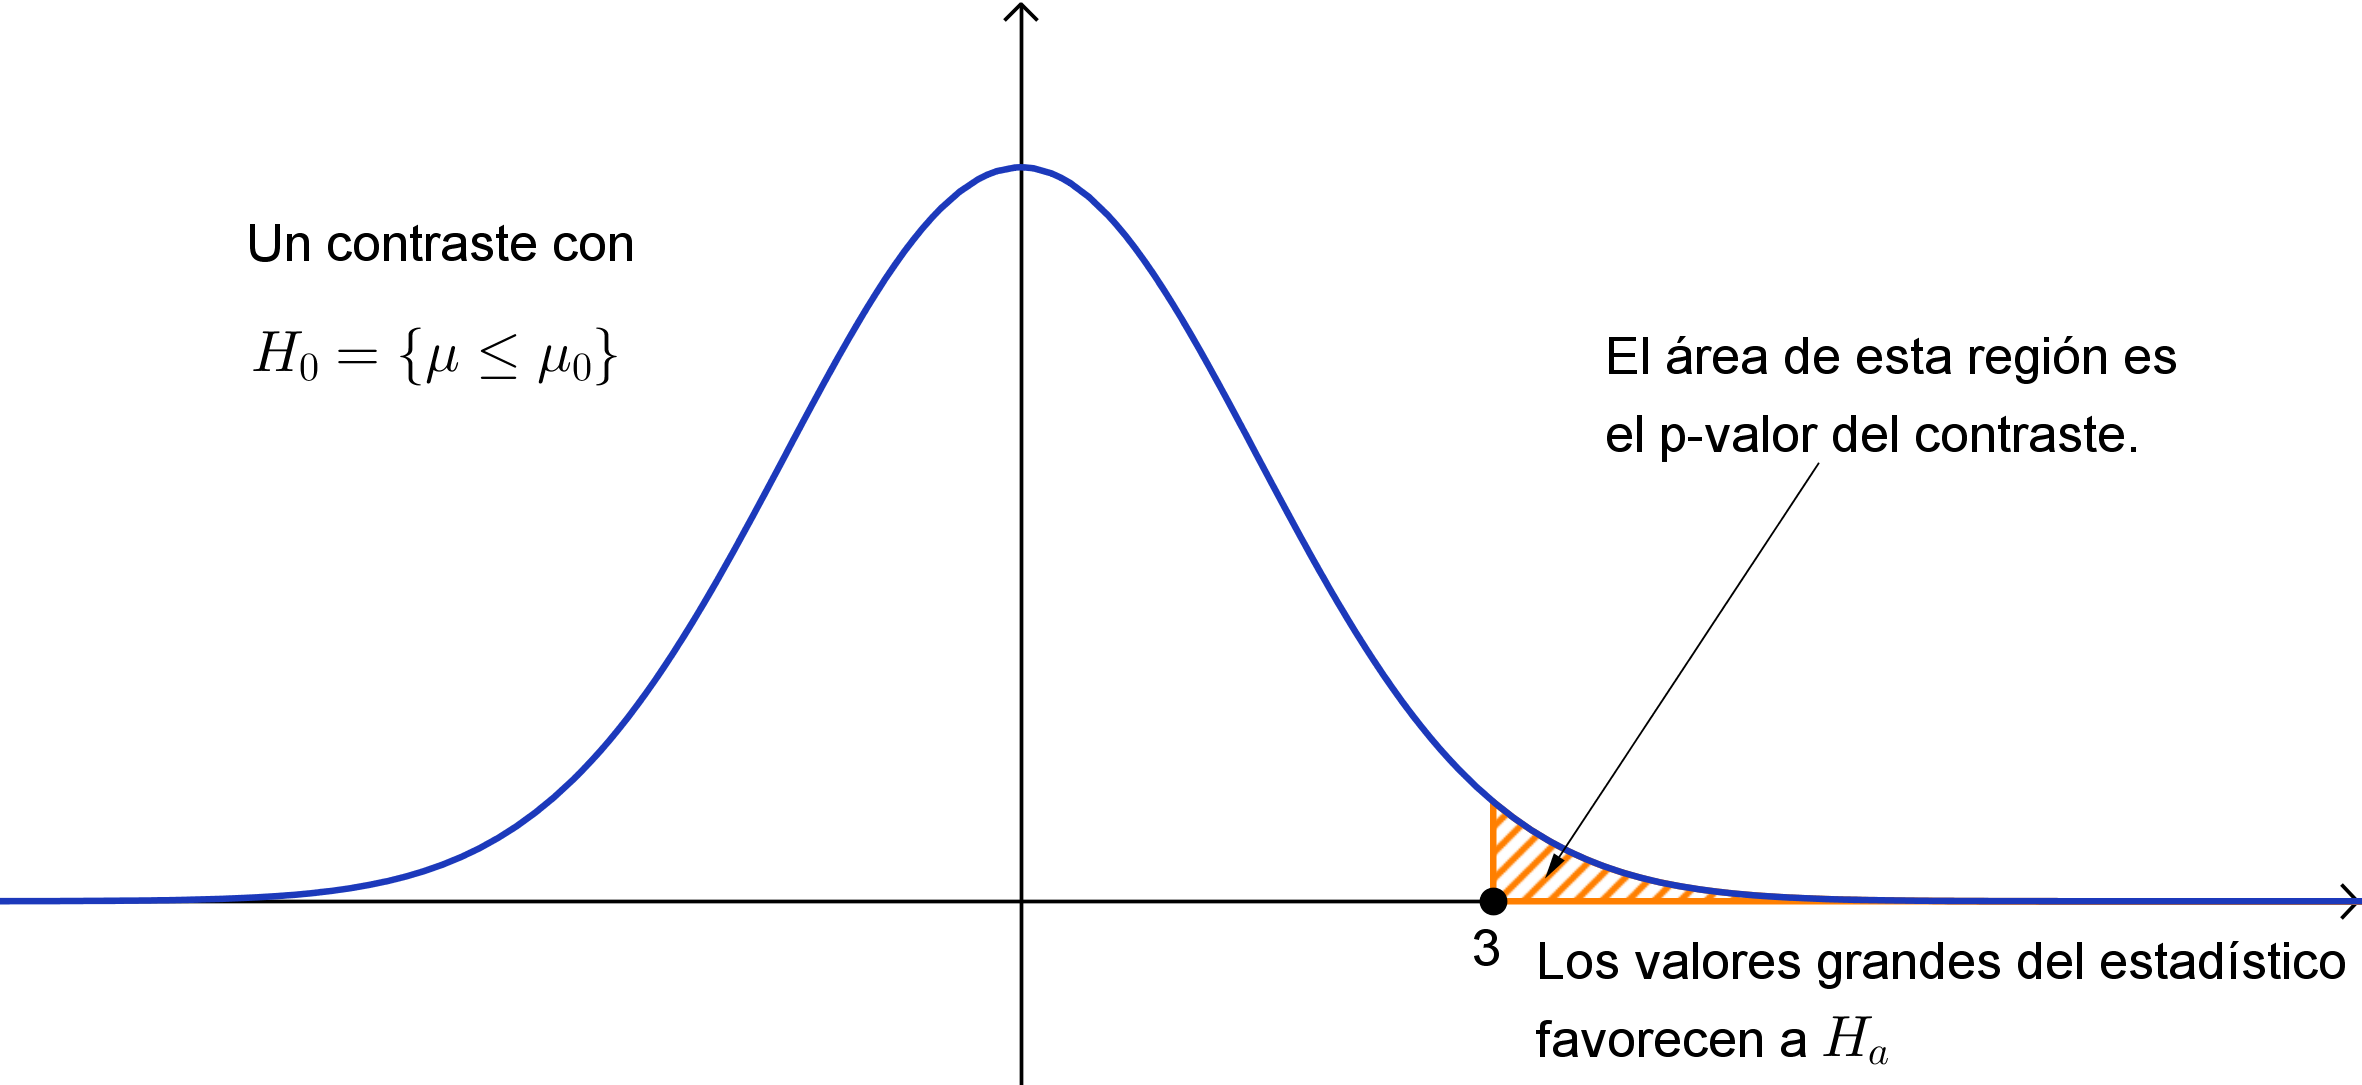
\includegraphics[width=13cm]{../fig/Cap07-PValorEjemploCanguros.png}
\end{enColor}
\begin{bn}
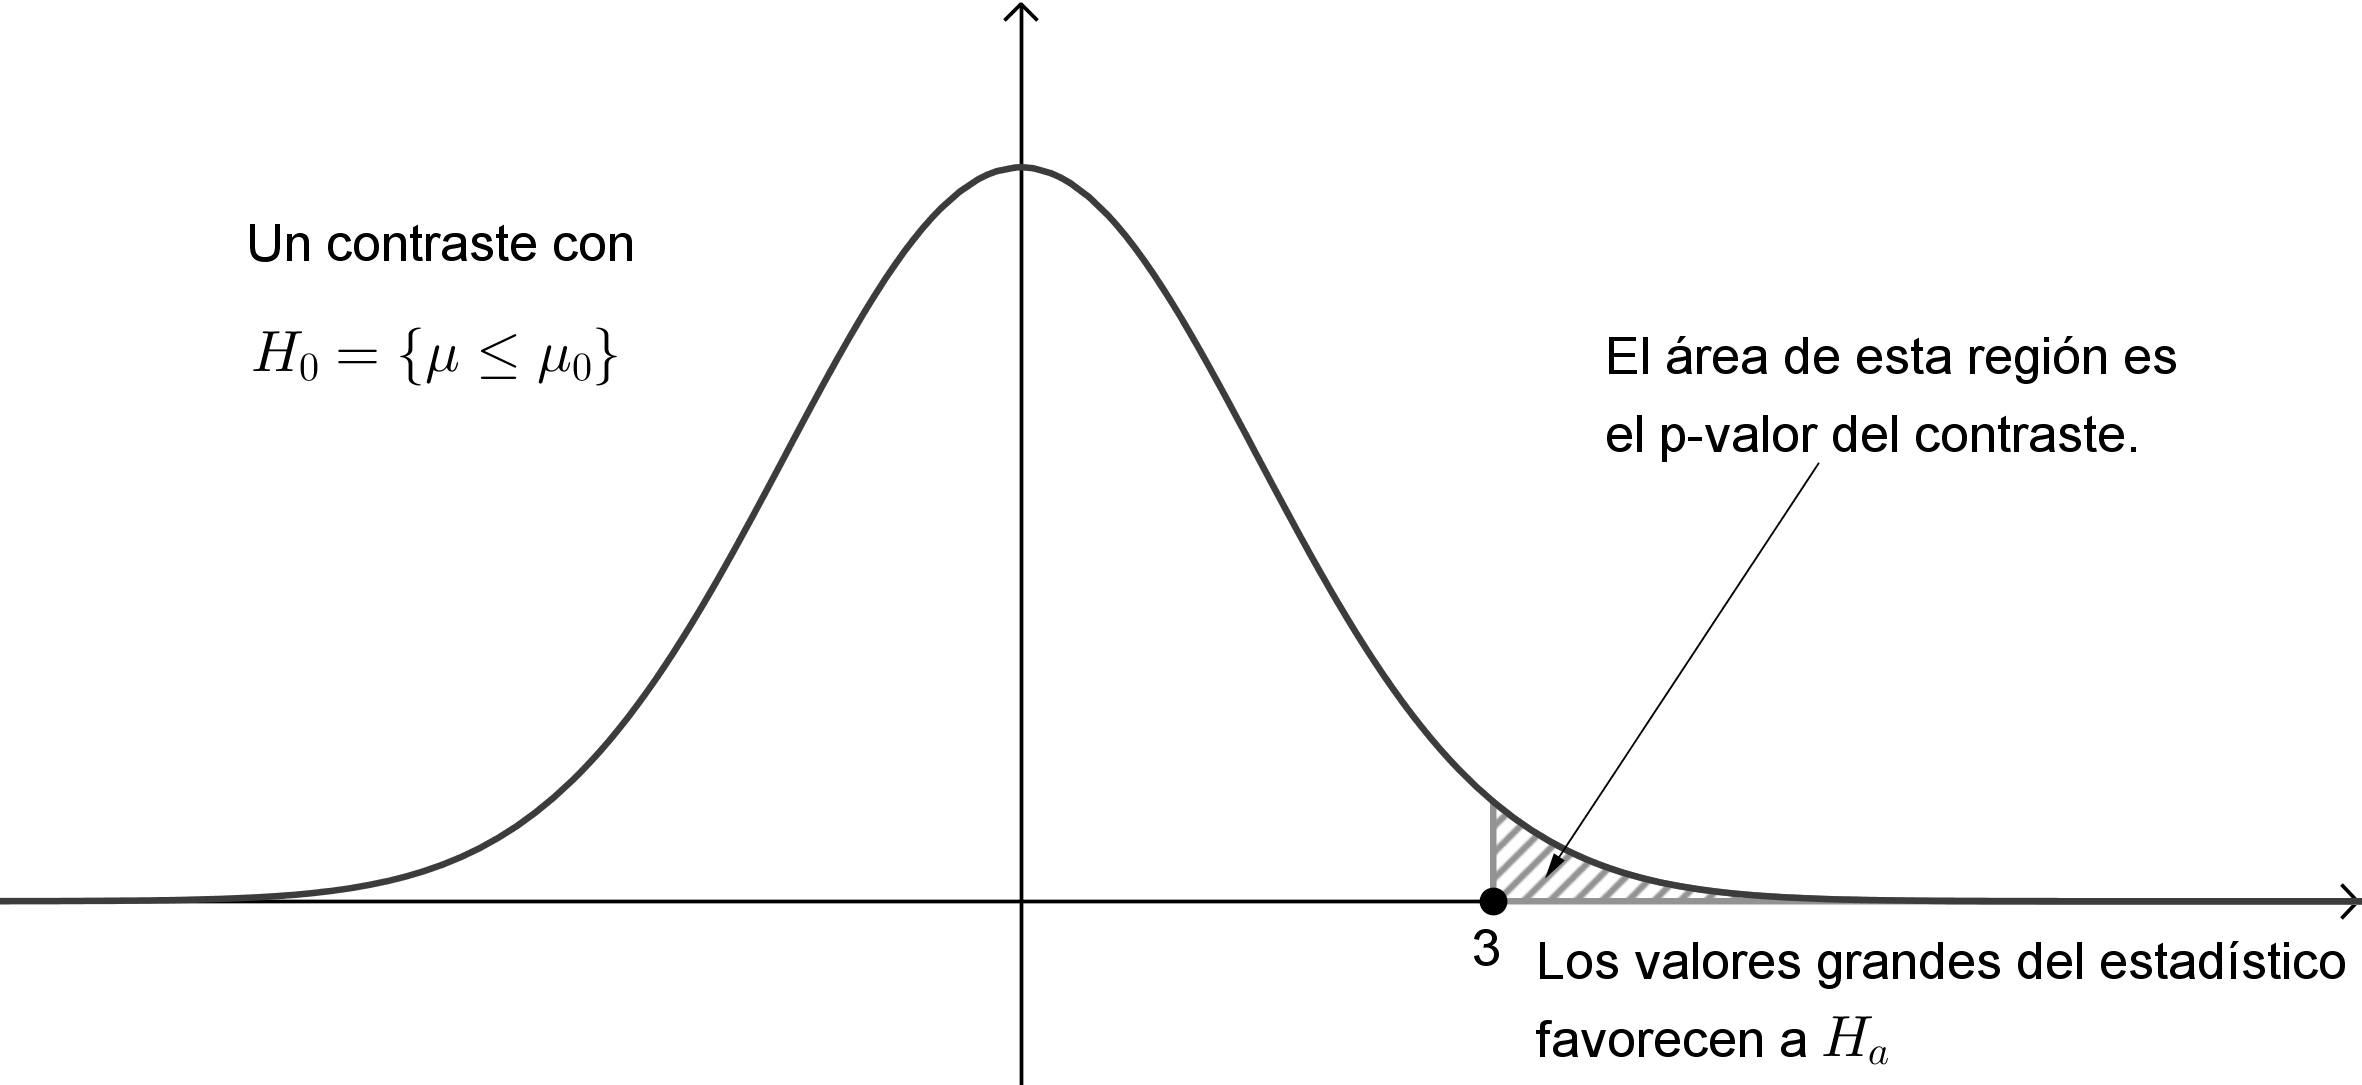
\includegraphics[width=13cm]{../fig/Cap07-PValorEjemploCanguros-bn.png}
\end{bn}
\caption{Cálculo del p-valor en el Ejemplo \ref{cap07:ejem:CangurosDepresivos03}.}
\label{cap07:fig:PValorEjemploCanguros}
\end{center}
\end{figure}

        Una vez identificado, el cálculo del p-valor es un problema directo de probabilidad muy sencillo. Usando el ordenador (recuerda que es una cola derecha), se obtiene:
        \[\mbox{p-valor}\approx 0.001350\]
        (con cuatro cifras significativas). Un p-valor siempre es una probabilidad, y responde a la pregunta que nos hacíamos al principio del contraste: ¿cómo de improbables le parecen los valores de nuestra muestra a alguien que cree que la hipótesis nula es cierta? En este ejemplo, el p-valor $0.0013$ que hemos obtenido significa que un partidario de la hipótesis nula esperaría que los canguros saltaran a esa altura aproximadamente una de cada mil veces. El partidario de la hipótesis alternativa no puede dejar de hacer notar que es bastante sospechoso que ese valor, tan poco frecuente, haya coincidido con la administración del {\em Pildorín Complex}...\qed
        \end{ejemplo}
\end{enumerate}
Como hemos visto, con el cálculo del p-valor hemos respondido a la pregunta inicial del contraste. Vamos a dar una definición más formal de este concepto, y a introducir algo más de la terminología que se utiliza en relación con los contrastes:
    \begin{center}
    \fcolorbox{black}{Gris025}{
    \begin{minipage}{12.5cm}
        %%%%%%%%%%%%%%%%%%%%%%%%%%%%%%%%%%%%%%%
        \begin{center}
        \subsubsection*{p-valor y contraste significativo.}
        \label{cap07:lugar:definicionPValor}
        \index{p-valor}
        \end{center}
       %%%%%%%%%%%%%%%%%%%%%%%%%%%%%%%%%%%%%%%
       El p-valor de un contraste de hipótesis  es la probabilidad de obtener los resultados de la muestra, u otros más favorables a la hipótesis alternativa $H_a$, cuando se supone que la hipótesis nula $H_0$ es cierta.\\
       Cuanto más pequeño sea el p-valor, más argumentos tenemos para rechazar la hipótesis nula. Por contra, con un p-valor grande, no podremos decir que los datos respaldan ese rechazo.\\
       Cuando el p-valor se considera suficientemente pequeño como para rechazar la hipótesis nula, decimos que es un {\sf contraste significativo}\index{contraste de hipótesis significativo}\index{significativo}. A veces también decimos, directamente, que el p-valor es significativo.
       %%%%%%%%%%%%%%%%%%%%%%%%%%%%%%%%%%%%%%%
    \end{minipage}}
    \end{center}
\quad\\[5mm]

Además, en el caso de un contraste como el del Ejemplo podemos concretar más. El p-valor es:
\begin{equation}\label{cap07:ecu:pValorMediaZColaDerecha}
\mbox{p-valor}=P\left(Z > \dfrac{\bar X-\mu_0}{\dfrac{s}{\sqrt{n}}}\right)=
P\left(Z > \mbox{estadístico}\right)
\end{equation}


En muchos casos, el contraste puede considerarse acabado con el cálculo del p-valor. Ya hemos obtenido la probabilidad, y ahora depende de nosotros decidir si esa probabilidad es suficientemente pequeña, como para decir que el contraste es significativo, y rechazar la hipótesis nula. Pero, en general, en cada disciplina científica hay un consenso establecido sobre cómo de pequeño debe ser el p-valor, para que el contraste se considere significativo. Para referirse a ese tipo de consenso existe una terminología bien establecida, que vamos a aprender a continuación.\\

\subsubsection*{Nivel de significación y region de rechazo.}

La terminología recuerda mucho a la que vimos en el caso de los intervalos de confianza. Si allí hablábamos de {\em nivel de confianza}, aquí vamos a definir un {\sf nivel de significación}\index{nivel de significación} $ns$\index{$ns=1-\alpha$, nivel de significación}, que típicamente tomará los valores $0.90$, $0.95$ o $0.99$. Y definimos, como en los intervalos de confianza, $\alpha=1-ns$. La práctica, habitual en muchos casos, consiste en fijar el nivel de significación {\em antes de realizar el contraste}. Por ejemplo, en muchos casos se establece $ns=0.95$, con lo que $\alpha=0.05$. A continuación se calcula el p-valor y se aplica la siguiente regla de decisión:

    \begin{center}
    \fcolorbox{black}{Gris025}{
    \begin{minipage}{12.5cm}
        %%%%%%%%%%%%%%%%%%%%%%%%%%%%%%%%%%%%%%%
        \begin{center}
        {\bf Contraste de hipótesis.}\\
        {\bf Método de decisión basado en el nivel de significación.}\\
        \end{center}
       %%%%%%%%%%%%%%%%%%%%%%%%%%%%%%%%%%%%%%%
       Dado un nivel de significación $ns$, sea $\alpha=1-ns$, y sea $p_0$ el p-valor de un contraste de hipótesis.
        \begin{itemize}
          \item Si $p_0<\alpha$, el contraste es significativo (rechazamos $H_0$).
          \item Si $p_0\geq \alpha$, el contraste no es significativo (no rechazamos $H_0$).
        \end{itemize}
       %%%%%%%%%%%%%%%%%%%%%%%%%%%%%%%%%%%%%%%
    \end{minipage}}
    \end{center}
Este esquema utiliza el p-valor para decidir si el contraste es o no significativo. Y el p-valor es una probabilidad. Concretamente, una {\em probabilidad} que se obtiene a partir del {\em valor} que el estadístico toma en la muestra. En Estadística, casi siempre se pueden abordar los problemas desde los valores, o desde sus correspondientes probabilidades. Ya vimos, al hablar de problemas directos e inversos, que podemos traducir valores en probabilidades y viceversa. Por ese motivo, hay otra forma de organizar la decisión del contraste de hipótesis, utilizando valores en vez de probabilidades. Este segundo esquema de trabajo, que desde luego es completamente equivalente al que ya hemos visto, utiliza la noción de {\sf región de rechazo}. Podemos definirla así:

    \begin{center}
    \fcolorbox{black}{Gris025}{
    \begin{minipage}{12.5cm}
        %%%%%%%%%%%%%%%%%%%%%%%%%%%%%%%%%%%%%%%
        \begin{center}
        {\bf Contraste de hipótesis.}\\
        {\bf Método de decisión basado en la región de rechazo.}\\
        \end{center}
       %%%%%%%%%%%%%%%%%%%%%%%%%%%%%%%%%%%%%%%
       Dado un nivel de significación $ns$, con $\alpha=1-ns$, la {\sf región de rechazo}\index{región de rechazo} (a ese nivel de significación) está formada por todos los valores del estadístico cuyos p-valores son menores que $\alpha$.\\
       Por lo tanto, si el valor del estadístico, calculado a partir de la muestra, pertenece a la región de rechazo, rechazamos la hipótesis nula $H_0$. Y, al revés, si no pertenece, no la rechazamos.
       %%%%%%%%%%%%%%%%%%%%%%%%%%%%%%%%%%%%%%%
    \end{minipage}}
    \end{center}

Vamos a ver como se obtiene la región de rechazo (para cierto nivel de significación) en el ejemplo de los canguros:
\begin{ejemplo}{(\bf Continuación del Ejemplo \ref{cap07:ejem:CangurosDepresivos06}).}
\label{cap07:ejem:CangurosDepresivos07}
    Vamos a suponer que fijamos un nivel de significación $ns=0.95$ (diremos, indistintamente, que es el 95\%). Por lo tanto $\alpha=1-0.95=0.05$, y como el p-valor que hemos obtenido es:
    \[p_0=\mbox{p-valor}\approx 0.001350\]
    se cumple
    \[p_0<\alpha\]
    y por lo tanto, rechazamos $H_0$ usando el p-valor. Vamos a continuación a determinar la región de rechazo para ese p-valor, y veremos que la conclusión, por este segundo método, es la misma. Para eso tenemos que resolver un problema inverso de probabilidad. Ya hemos visto, anteriormente en este ejemplo, que los valores del estadístico que favorecen a la hipótesis nula, son los de la cola derecha de la normal estándar. Así que el problema inverso que hay que resolver, para determinar la región de rechazo correspondiente a $\alpha$,  es este:
    \begin{center}
    {\em ¿Cuál es el valor $z_{\alpha}$ que cumple $P(Z\geq z_{\alpha})=\alpha$?}
    \end{center}
    Si la notación te recuerda a la de los valores críticos (ver página \pageref{cap06:ecu:DefinicionValorCriticoZ}), es porque la definición es la misma. El valor $z_{\alpha}$, que define la región de rechazo en este ejemplo, es precisamente el valor crítico correspondiente de $Z$. Lo calculamos (usando el ordenador; recuerda que es una cola izquierda) y obtenemos:
    \[z_{\alpha}\approx 1.645\]
    (cuatro cifras significativas). Por lo tanto, la región de rechazo la forman los valores del estadístico que cumplan:
    \[\dfrac{\bar X-\mu_0}{\dfrac{s}{\sqrt{n}}} > z_{\alpha}\]
    La región de rechazo, para este tipo de contraste, aparece en la Figura \ref{cap07:fig:RegionRechazoNormalColaDerecha} (pág. \pageref{cap07:fig:RegionRechazoNormalColaDerecha}).
    Nosotros hemos obtenido (antes, en la página \pageref{cap07:ejem:CangurosDepresivos04}) un valor del estadístico igual a $3$. Así,  puesto que
    \[3 > 1.645,\]
    el valor del estadístico pertenece a la región de rechazo, y la conclusión de este método es la misma (como tiene que ser siempre): rechazamos la hipótesis nula $H_0$.\qed
\end{ejemplo}
En este ejemplo hemos visto que la región de rechazo
\begin{equation}
\label{cap07:ecu:RegionRechazoMediaZColaDerecha}
R=\left\{\dfrac{\bar X-\mu_0}{\dfrac{s}{\sqrt{n}}} > z_{\alpha}\right\}
\end{equation}
se define (y se calcula) con independencia de que la hipótesis nula $H_0$ sea cierta o no. Pero si además sucede que $H_0$ es cierta, entonces la distribución del estadístico
     \[\dfrac{\bar X-\mu_0}{\frac{s}{\sqrt{n}}}\]
es realmente la normal estándar. En ese caso, si obtenemos un valor de este estadístico en la región de rechazo (porque, por ejemplo, hemos tenido {\em mala suerte} con nuestra muestra), habremos rechazado la hipótesis nula, {\em a pesar de que es cierta}. Es decir, habremos cometido un error de tipo I. Y, puesto que hemos usado $z_{\alpha}$ para construir la región de rechazo $R$,  la probabilidad de obtener alguno de esos valores en $R$ es igual a $\alpha$\footnote{Aquí, precisamente en esta frase, es donde usamos el hecho de que $H_0$ es cierta.}. Por tanto, comprobamos que:
    \[\alpha=P(\mbox{error de tipo I})=
    P(\mbox{rechazar }H_0 | H_0\mbox{ es cierta})=
    P(\mbox{falso positivo})\]
Eso justifica la elección de notación que hicimos en Ecuación \ref{cap07:ecu:AlfaErrorTipoI} (pág. \pageref{cap07:ecu:AlfaErrorTipoI}). Análogamente, el valor
    \[\beta=P(\mbox{error de tipo II})=
    P(\mbox{no rechazar }H_0 | H_a\mbox{ es cierta})=
    P(\mbox{falso negativo})\]
es la probabilidad
%de la región de rechazo de la hipótesis alternativa. Es decir, la probabilidad
de no rechazar $H_0$ (y rechazar la hipótesis alternativa), {\em a pesar de que $H_a$ es cierta}. Los dos tipos de errores van fuertemente emparejados. A primera vista podríamos pensar que lo mejor es tratar de hacer ambos errores pequeños simultáneamente. Pero esto es, en general, inviable, porque al disminuir la probabilidad de cometer un error de tipo I (al disminuir $\alpha$) estamos aumentando la probabilidad de cometer uno de tipo II (aumentamos $\beta$). En la Sección \ref{cap07:sec:PotenciaContraste} daremos más detalles.

Como hemos dicho, la decisión sobre el tipo de error que queremos evitar depende mucho del contexto: los errores de tipo I se consideran más relevantes cuando, como en nuestro ejemplo, se está estudiando un nuevo procedimiento terapéutico, o se propone una nueva teoría. En ambos casos, tendemos a ser conservadores, protegiendo el conocimiento previo. Sin embargo, en otras aplicaciones, como los ejemplos de control de calidad, seguridad alimentaria, o estudios medio ambientales a los que hemos aludido antes, los errores de tipo II son los más preocupantes.

\subsubsection*{Rechazamos hipótesis, pero nunca las {\em aceptamos}.}

Ahora que ya hemos desarrollado algo mejor el lenguaje de los contrastes de hipótesis, antes de seguir adelante queremos detenernos en un aspecto relativo precisamente a la terminología que usaremos. Hemos hablado ya varias veces de {\em rechazar} una hipótesis, cuando los datos de los que disponemos la hacen inverosímil. A la vista de esa frase, muchos recién llegados a la Estadística concluyen que ``si rechazamos la hipótesis nula $H_0$, entonces es que {\em aceptamos} la hipótesis alternativa $H_a$''. Hemos destacado el verbo {\em ``aceptar''} porque queremos señalar que lo consideraremos un {\em verbo prohibido} en el contexto del contraste de hipótesis. Por, al menos, las dos siguientes razones:
\begin{itemize}
  \item La primera es de índole más filosófica, y tiene que ver con el hecho de que uno de los objetivos básicos del método científico es disponer de herramientas para demostrar que una afirmación es falsa, incompatible con los datos. Las hipótesis no se ``aceptan'', en el sentido de pasar a considerarse ciertas, como podría considerarse cierto un teorema en Matemáticas, una vez demostrado. No existe, en la Ciencia, el equivalente de la demostración en Matemáticas. Las hipótesis se consideran siempre provisionales, a la espera de que nuevos datos puedan contradecirlas alguna vez, y obligarnos a formular una nueva teoría.
  \item La segunda razón es mucho más concreta y, desde nuestro punto de vista, más contundente. Si repasas los pasos que hemos dado para hacer el contraste de hipótesis del Ejemplo \ref{cap07:ejem:CangurosDepresivos03}, verás que no hay nada que nos hubiera impedido hacer un contraste de hipótesis usando una muestra de tamaño, pongamos,  $n=5$. Sugerimos al lector que rehaga las cuentas de ese ejemplo con $n=5$ y manteniendo todos los demás valores iguales. En ese caso se obtiene un p-valor aproximadamente igual a $0.25$ (recuerda que en el ejemplo original, con $n=100$, se obtenía como p-valor 0.001350). Un p-valor tan grande como $0.25$ significa que nuestros datos son los que, usando la hipótesis nula, esperaríamos observar una de cada cuatro veces. Y por lo tanto no ponen a esa hipótesis nula $H_0$ en entredicho (como si hacía el p-valor para $n=100$). Es decir, que si, en el Ejemplo \ref{cap07:ejem:CangurosDepresivos03}, nuestra muestra hubiera sido de tamaño $n=5$, no hubiéramos rechazado la hipótesis nula. ¿Significa eso que {\em aceptamos} la hipótesis nula, en el sentido de pensar que es {\em verdadera}? {!`}Ni mucho menos! Hemos usado una muestra muy pequeña, así que no parece muy sensato basar nuestro concepto de lo que es {\em cierto} en una evidencia experimental tan escasa. La única conclusión razonable, en tal caso, es la formulación que se hace habitualmente en Estadística: con esos datos (los de la muestra con $n=5$) no tenemos base experimental para rechazar $H_0$ y no hablamos (de hecho, no volveremos a hablar en todo el resto del curso) de {\em aceptar} la hipótesis).
\end{itemize}

\subsubsection*{Advertencia sobre el (ab)uso del p-valor. La $d$ de Cohen.}
\label{cap07:subsubsec:AdvertenciaAbusoPValor}

Enlazando con la discusión anterior, queremos prevenir al lector contra una práctica que puede llegar a resultar en una aplicación imprecisa de los métodos de la Estadística, y a extraer conclusiones poco sólidas. Hemos explicado cómo se usa el p-valor para decidir si rechazamos una hipótesis (cuando el contraste es significativo) y en la Sección \ref{cap07:sec:ContrasteHipotesisPasoaPaso} hemos descrito un modus operandi {\em paso a paso} para hacer un contraste de hipótesis. Vuelve a repasar esa sección para refrescar cuáles son esos pasos. Como verás, el resultado es un mecanismo de decisión sencillo de aplicar, casi mecánico, susceptible de suscitar acuerdo entre los científicos y cuya aplicación, en principio, está al alcance de cualquiera (de hecho, se puede programar el procedimiento en un ordenador). Eso explica la popularidad del método de contraste usando el p-valor desde que Fisher lo inventó en 1925. La sencillez de aplicación hizo que ese procedimiento mecánico antes descrito se generalizara rápidamente. El riesgo que se corre, como siempre que se mecaniza un procedimiento, es el de aplicarlo sin tener en cuenta otras consideraciones que pueden influir en la interpretación del resultado del contraste.  Recientemente la comunidad científica ha reabierto el debate sobre el uso correcto de esta técnica. Por ejemplo, en el momento de escribir esto (Junio de 2016) la American Statistical Association (Asociación Americana de Estadística) ha decidido tomar cartas en el asunto y encargar a un selecto panel de expertos un artículo sobre el uso (y abuso) del p-valor. Puedes ampliar la información sobre este tema en los artículos  \cite{wasserstein2016asa} y \cite{nuzzo2014statistical}, ambos escritos de forma muy accesible  y cuya lectura recomendamos.

En cualquier caso, aquí queremos destacar un problema asociado al uso del p-valor que nos parece especialmente relevante. Como hemos visto en las secciones anteriores, proporcionar el p-valor de un contraste, sin acompañarlo del tamaño de la muestra que se ha usado, resta mucho valor a las conclusiones que se puedan extraer de ese p-valor aisladamente.
Pero, incluso cuando la muestra es grande y el contraste es significativo (con un p-valor suficientemente pequeño), todavía es necesario prestar atención a otros aspectos del problema. El siguiente ejemplo trata de ilustrar esta discusión.
\begin{ejemplo}{\bf (Continuación del Ejemplo \ref{cap07:ejem:CangurosDepresivos03}).}
\label{cap07:ejem:AbusoPValor}
Supongamos que, en el estudio sobre el efecto del {\em Pildorín Complex} del Ejemplo \ref{cap07:ejem:CangurosDepresivos03}, hubiéramos medido una media muestral
\[\bar X=2.52 cm\]
Recordando que, en aquel ejemplo, era $\mu_0=2.5$. Con una diferencia tan pequeña entre $\bar X$ y $\mu_0$, seguramente el lector piense que el contraste de hipótesis no puede ser significativo. Pero no hemos dicho aún cual es el tamaño de la muestra en la que se obtuvo ese valor de $\bar X$. Supongamos que ese valor se obtuvo con una muestra de nada menos que $n=10000$ canguros depresivos. Entonces, suponiendo que el valor de $s=0.5$ no ha cambiado, primero calculamos el estadístico:
        \[
         Z=\dfrac{\bar X-\mu_0}{\dfrac{s}{\sqrt{n}}}=
         \dfrac{2.52-2.5}{\dfrac{0.5}{\sqrt{10000}}}=\dfrac{0.02}{0.005}=4.
         \]
Y ahora, usando el ordenador, calculamos el p-valor (recuerda la Ecuación \ref{cap07:ecu:pValorMediaZColaDerecha}, pág. \pageref{cap07:ecu:pValorMediaZColaDerecha}):
\[\mbox{p-valor}=P\left(Z > \mbox{estadístico}\right)\approx 0.00003167\]
Es un p-valor muy pequeño, más pequeño de hecho que el que obtuvimos en la versión original del Ejemplo \ref{cap07:ejem:CangurosDepresivos03}. ¿Cómo es posible, si $\mu_0$ y $\bar X$ son prácticamente iguales? Pues porque el tamaño de la muestra es muy grande.
\qed
\end{ejemplo}
La primera lección que debemos extraer de este ejemplo es que cualquier diferencia entre $\bar X$ y $\mu_0$ puede llegar a ser significativa, si se considera una muestra suficientemente grande (gracias al Teorema Central del Límite). Porque, al fin y al cabo, $n$ divide al denominador del estadístico.
Y eso, a su vez, implica que un p-valor pequeño y una muestra grande (de hecho, especialmente si van juntos) no es a menudo el final de la historia.

La segunda, y más importante, lección que debemos aprender aquí, es que hay una diferencia esencial entre que un resultado sea {\em estadísticamente significativo} y que lo podamos considerar {\sf científicamente relevante}\index{relevante, resultado}\index{científicamente relevante, resultado}. Este segundo concepto es, sin duda, el que nos interesa en la mayor parte de las ocasiones. Y, como decimos, para juzgar si un resultado es científicamente relevante, es necesario acompañar el p-valor con, obligatoriamente, el tamaño de la muestra, y, al menos, alguna información adicional sobre el {\sf tamaño del efecto}\index{efecto, tamaño del}\index{tamaño del efecto} (en inglés, {\em effect size})\index{effect size}. ¿Qué significa eso del tamaño del efecto? Se trata de dar una medida de como de lejos están $\bar X$ y $\mu_0$, en una escala que sea realista desde el punto de vista de la población que estamos analizando. Una medida habitual del tamaño del efecto es el siguiente valor:
\begin{equation}\label{cap07:ecu:CohenD}
d =\dfrac{\bar X-\mu_0}{s}
\end{equation}
llamado la {\sf $d$ de Cohen}\index{Cohen, $d$ de}\index{$d$ de Cohen}, que, sin duda, te recordará al estadístico del contraste. Pero verás que en esta definición ha desaparecido el tamaño $n$ de la muestra, de manera que aquí (pensando en $s$ como un estimador de $\sigma$), lo que estamos haciendo es muy parecido a una tipificación de $\bar X$ con respecto a la normal que describe a la población. Eso nos permite interpretar los valores de $d$ como una medida de si, realmente, el valor $\bar X$ se aleja de $\mu_0$ de una manera relevante. Un valor de $d$ inferior a $0.2$ apunta a que la diferencia no es relevante. Por otra parte, cuando la diferencia es relevante, el valor de $d$ que se obtiene suele ser mayor que $0.8$. Pero cuidado: un valor grande de $d$ no es, por sí mismo, una garantía de que la diferencia es relevante. Siempre hay que tratar de asegurarse por otros medios (por ejemplo, usando intervalos de confianza) y, en cualquier caso, tener en cuenta la opinión sobre la relevancia de esos datos, procedente de un experto en el problema de que se trate.
\begin{ejemplo}{\bf (Continuación del Ejemplo \ref{cap07:ejem:AbusoPValor}).}
\label{cap07:ejem:AbusoPValor2}
En el caso de la muestra con $\bar X=2.52$, la $d$ de Cohen es:
\[d=\dfrac{\bar X-\mu_0}{s}=\dfrac{2.52-2.5}{0.5}=\dfrac{0.02}{0.5}=0.04\]
así que el tamaño del efecto se podría considerar como irrelevante desde el punto de vista científico. Por contra, en el ejemplo original, tenemos
\[d=\dfrac{\bar X-\mu_0}{s}=\dfrac{2.65-2.5}{0.5}=\dfrac{0.15}{0.5}=0.3,\]
así que el tamaño del efecto es, en este caso, (bastante) moderadamente relevante. En cualquier caso, fíjate en que es siete veces más relevante que el otro resultado, a pesar de contar con una muestra mucho menor.
\qed
\end{ejemplo}
La $d$ de Cohen no es la única forma de medir el tamaño del efecto en un contraste, pero por el momento nos vamos a conformar con esto, subrayando que lo importante es entender que el p-valor, aislado del resto de la información, no puede considerarse un criterio suficiente para juzgar un resultado científico.

\paragraph{Comentarios adicionales sobre el p-valor.}

Antes de seguir adelante es importante remarcar algo: en absoluto pretendemos decir que la inferencia basada en el p-valor carezca de sentido. Por el contrario, se trata de una herramienta muy potente y, en muchos casos,  perfectamente legítima.
En este apartado hemos centrado nuestra atención en el riesgo de abusar del p-valor, confundiendo significación estadística con relevancia científica. Pero hay otro aspecto del uso del p-valor en el que queremos fijarnos ahora. El p-valor, recordémoslo una vez más, es la probabilidad de obtener los valores muestrales {\em si la hipótesis nula $H_0$ es cierta.} Pero si hacemos el contraste y, usando el p-valor, rechazamos la hipótesis nula, entonces {\em esa misma interpretación del p-valor como probabilidad de los valores muestrales deja de tener validez}. El p-valor sólo se puede interpretar así mientras se mantiene la validez de la hipótesis nula.

¿Qué podemos decir, entonces, en términos de probabilidad, cuando rechazamos la hipótesis nula? Si $H_0$ es falsa, entonces $H_a$ es cierta. Así que la discusión, en este caso, tiene que ver con la probabilidad de, a partir de la muestra, rechazar $H_0$, cuando $H_a$ es cierta. Y eso nos lleva directamente a la noción de {\em potencia} del contraste.


\section{Potencia de un contraste y tamaño de la muestra.}
\label{cap07:sec:PotenciaContraste}

%\noindent{\bf Atención:} Esta sección puede omitirse en una primera lectura del capítulo.

El concepto de {\sf potencia} de un contraste de hipótesis, que hemos mencionado en la página \pageref{cap07:ecu:BetaErrorTipoII}, está muy relacionado con esta discusión. Recordemos que hemos dicho que la potencia es:
\[\mbox{potencia } =  1-\beta=1-P(\mbox{error de tipo II})=\]
\[=1-P(\mbox{no rechazar }H_0 | H_a\mbox{ es cierta})=P(\mbox{rechazar }H_0 | H_a\mbox{ es cierta}).\]
Por lo tanto la potencia es la probabilidad de {\em no cometer} un error de tipo II. Es decir, es la probabilidad de acertar al rechazar $H_0$. Pero esta no es una definición que permita, por si misma, calcular un valor de la potencia. Para poder calcular un número, necesitamos precisar un poco más. Veamos por qué.

En general, la potencia va estrechamente ligada al tamaño de la muestra, que, además, es uno de los pocos valores sobre los que el experimentador puede, en ocasiones, ejercer algún control. Es razonable esperar que cuanto más grande sea la muestra, más fácil sea detectar una hipótesis nula falsa. Pero la potencia también depende de la discrepancia mínima que queremos que el contraste sea capaz de detectar. Por ejemplo, en el contraste sobre medias que hemos visto, para un tamaño de muestra fijo, es tanto más fácil rechazar $H_0$, cuanto mayor sea la diferencia entre $\mu$ y $\mu_0$. Y, recíprocamente, para una diferencia entre $\mu$ y $\mu_0$ dada, cuanto mayor sea el tamaño de la muestra, más potencia tendrá el contraste. Vamos a ver como intervienen estos ingredientes en el cálculo de la potencia para el Ejemplo \ref{cap07:ejem:CangurosDepresivos01}.

\begin{ejemplo}{\bf (Continuación del Ejemplo \ref{cap07:ejem:CangurosDepresivos03}).}
\label{cap07:ejem:CalculoPotenciaEjemploCanguros}
    La hipótesis nula de ese ejemplo era
    \[H_0: \{\mu\leq \mu_0\},\]
    con $\mu_0=2.5$. Para calcular la potencia, suponemos que la hipótesis nula es falsa. Eso quiere decir que la media es mayor que $\mu_0$. Pero saber que es mayor no es suficientemente concreto. Tenemos que fijar un valor. Supongamos que la media real es $\mu = 2.6$, de manera que la diferencia es $\delta=\mu-\mu_0=0.1$. Ahora tenemos que calcular la probabilidad $1-\beta$ de rechazar $H_0$. Cuando hacemos el contraste (con nivel de significación $ns=1-\alpha$), decimos que la región de rechazo la forman los valores del estadístico que cumplan:
    \[\dfrac{\bar X-\mu_0}{\dfrac{s}{\sqrt{n}}} > z_{\alpha}\]
    Pero no podemos utilizar esta expresión para calcular probabilidades, porque se basa en la suposición de que $H_0$ es cierta. {!`}Y precisamente, ahora estamos suponiendo que es falsa! En particular, el estadístico
    \[\dfrac{\bar X-\mu_0}{\dfrac{s}{\sqrt{n}}}\]
    {\bf no} se distribuye según una normal estándar. Como hemos supuesto que la media real es $\mu=2.6$, el estadístico que realmente se distribuye según $Z$ es:
    \[\dfrac{\bar X-\mu}{\dfrac{s}{\sqrt{n}}},\]
    y este es el que debemos usar, si queremos calcular probabilidades correctas. La potencia $1-\beta$ es, entonces, la probabilidad ({!`}correctamente calculada!):
    \[
       \mbox{potencia } =  P\left(\left.\dfrac{\bar X-\mu_0}{\dfrac{s}{\sqrt{n}}} > z_{\alpha}\right|
        \rule{0cm}{1cm}\stackrel{H_a\mbox{ es cierta, y}}{\mbox{ la media es }\mu=2.6}\right),
    \]
    porque cuando se cumpla esa desigualdad es cuando rechazaremos la hipótesis nula. La idea clave es que hay que calcular correctamente la probabilidad, así que tenemos que reescribir esta desigualdad para que aparezca el estadístico con $\mu$ en lugar de $\mu_0$, porque ese es el que permite cálculos correctos de probabilidad. Hacemos una pequeña manipulación algebraica:
        \[
            P\left(\left.\dfrac{\bar X-\mu+(\mu-\mu_0)}{\dfrac{s}{\sqrt{n}}}> z_{\alpha}\right|
            H_a\mbox{ cierta} \right)=
            P\left(\left.
            \dfrac{\bar X-\mu}{\dfrac{s}{\sqrt{n}}}+\dfrac{\mu-\mu_0}{\dfrac{s}{\sqrt{n}}}
            > z_{\alpha}\right|
            H_a\mbox{ cierta}\right)
        ,\]
    o, lo que es lo mismo:
        \[
            P\left(\left.
            \dfrac{\bar X-\mu}{\dfrac{s}{\sqrt{n}}}
            > z_{\alpha}-\dfrac{\delta}{\dfrac{s}{\sqrt{n}}}\right|
            \rule{0cm}{1cm}\stackrel{H_a\mbox{ es cierta,}}{\mbox{ y la media es }\mu}\right)
        .\]
    Esta última expresión es justo lo que necesitábamos, porque en la parte izquierda aparece el estadístico con $\mu$, del que (al ser $H_a$ cierta) sabemos que se distribuye según la normal estándar. Así que ahora podemos sustituir los valores de este ejemplo
    \[\alpha=0.05,\quad \delta=0.1,\quad  s=0.5,\quad  n=100,\]
    y afirmar que:
    \[\mbox{potencia}=1-\beta=P\left(
            Z> z_{0.05}-\dfrac{0.1}{\dfrac{0.5}{\sqrt{100}}}\right).
    \]
    Las cuentas pueden hacerse en el ordenador
    %(con R usamos {\tt qnorm} para calcular $z_{\alpha}$, y luego {\tt pnorm} para obtener $\beta$)
    y se obtiene
    \[\mbox{potencia}\approx 0.6388\]
    (cuatro cifras significativas). Es decir, que la potencia de este contraste, con $\delta=0.1$, $s=0.5$ y $n=100$ es aproximadamente del 64\%. Es una potencia relativamente baja, se suelen buscar potencias cercanas al 80\% como poco. Una forma de aumentar la potencia, como hemos dicho, sería usar una muestra más grande.
    \qed
\end{ejemplo}
En este ejemplo hemos obtenido
\begin{equation}\label{cap07:ecu:EcuacionPotenciaContrasteMediaConZ}
    \mbox{potencia}=1-\beta=P\left(Z> z_{\alpha}-\dfrac{\delta}{\dfrac{s}{\sqrt{n}}}\right).
\end{equation}
para el contraste de la hipótesis nula
\[H_0=\{\mu\leq \mu_0\}\]
con muestra grande. Además $\delta=\mu-\mu_0$ representa la diferencia de $\mu_0$ la media real $\mu$. Normalmente se interpreta $\delta$ como la diferencia mínima que es capaz de detectar (considerando, en tal caso, la potencia como un dato prefijado).

Esta expresión muestra que la potencia del contraste depende de $\alpha$ (a través del valor crítico $z_{\alpha}$) y también depende de la cantidad:
\[\dfrac{\delta}{\dfrac{s}{\sqrt{n}}}.\]
Para otros contrastes se obtienen fórmulas similares, en general más complicadas. También podemos usar esa expresión para concretar nuestra afirmación de que al tratar de reducir $\alpha$ estaríamos (disminuyendo la potencia y, por tanto,) aumentando $\beta$. En efecto, si en lugar de $\alpha=0.05$ usamos, por ejemplo, $\alpha=0.01$, tendríamos $z_{0.01}>z_{0.05}$. Así que en la desigualdad que aparece dentro de la función probabilidad tenemos que calcular la probabilidad de una cola derecha de $Z$ más pequeña. La potencia disminuye, y $\beta$ aumenta. A menudo, y como resumen, suele suponerse que la potencia de un contraste de hipótesis cumple una relación de este tipo:
    \begin{equation}
    \label{cap07:ecu:relacionGenericaPotencia}
    \mbox{potencia}=1-\beta = K\, \dfrac{\delta\,\sqrt{n}\,\alpha}{\sigma}
    \end{equation}
para alguna constante de proporcionalidad $K$.  Esta fórmula es {\em aproximada y puramente descriptiva}, ya que en cada caso concreto los detalles pueden ser distintos. Pero la idea básica, para la que sirve la Ecuación \ref{cap07:ecu:relacionGenericaPotencia}, es para recordarnos que la potencia tiene estas propiedades:
\begin{itemize}
  \item Como hemos visto, la potencia aumenta con $\alpha$, que es la probabilidad de un error de tipo I. Y al aumentar la potencia (que es $1-\beta$), también disminuye $\beta$, la probabilidad de un error de tipo II.
  \item Aumenta con el tamaño de la muestra, concretamente como la raíz del tamaño de la muestra.
  \item Disminuye con $\sigma$. Cuanto más dispersa sea la población, menor será la potencia, claro.
  \item Aumenta con $\delta$. Si $H_a$ es cierta, cuanto más lejos esté la media real de la media $\mu_0$, más fácil es detectar esa diferencia, y rechazar $H_0$.
\end{itemize}

\subsection{Estimación del tamaño necesario de la muestra.}
\label{cap07:subsec:EstimacionTamannoMuestra}


Las ecuaciones de potencia tienen una forma que se puede describir genéricamente mediante la Ecuación \ref{cap07:ecu:relacionGenericaPotencia} que hemos visto. Es decir, son de la forma:
\[\mbox{potencia}=1-\beta = K\, \dfrac{\delta\,\sqrt{n}\,\alpha}{\sigma}\]
Insistimos en que esta relación es una representación simplificada de un conjunto de ecuaciones que, en cada caso particular, tienen una forma más o menos complicada. Esas ecuaciones de potencia se usan a menudo para {\em estimar} el tamaño de la muestra que sería necesaria para conseguir algún objetivo concreto que el experimentador se haya propuesto al diseñar el experimento. La Ecuación \ref{cap07:ecu:relacionGenericaPotencia} muestra que la potencia depende de cuatro cantidades (sin contar la constante $K$). Si incluimos la propia potencia, hay cinco variables en la ecuación. Dicho de otro modo, podemos fijar cuatro de ellas, y despejar la quinta. En particular, y dado que el tamaño de la muestra es una de las pocas cosas que el experimentador puede, a veces, controlar mediante el diseño, se suele utilizar este tipo de ecuaciones para calcular el mínimo tamaño $n$ necesario de la muestra en función de $\delta$, $\alpha$, $\beta$ y $\sigma$, que se consideran  como valores dados. Para fijar ideas, supongamos,  por ejemplo, que queremos trabajar con un nivel de significación del $95\%$, y que el contraste tenga una potencia del $80\%$ (es una cifra típica para la potencia, similar al $95\%$ para el nivel de significación). Además, para seguir adelante, necesitamos una estimación de $\sigma$, la  desviación típica de la población. Naturalmente, la obtendremos de una muestra, usando $s$ como estimador de $\sigma$. Y, al igual que hicimos en el caso de los intervalos de confianza (ver la Sección \ref{cap06:subsec:CalculoTamannoMuestra}, pág. \pageref{cap06:subsec:CalculoTamannoMuestra} y también la discusión de la página \pageref{cap06:subsubsec:DeterminacionTamannoMuestraParaMuConSigmaDesconocida}), se suele utilizar un valor obtenido en algún {\em estudio piloto}, con una muestra de un tamaño más reducido, o de alguna otra información previa sobre la dispersión de la población de la que se disponga.
Veamos un caso concreto, con los datos del ejemplo de los canguros depresivos que venimos usando en este capítulo.
\begin{ejemplo}{\bf (Continuación del Ejemplo \ref{cap07:ejem:CalculoPotenciaEjemploCanguros}).}
\label{cap07:ejem:CalculoPotenciaEjemploCanguros2}
Vamos a usar los datos del anterior Ejemplo \ref{cap07:ejem:CalculoPotenciaEjemploCanguros} (pág. \pageref{cap07:ejem:CalculoPotenciaEjemploCanguros}) como punto de partida (como {\em estudio piloto}), para averiguar el tamaño muestral $n$ necesario para realizar un contraste de hipótesis con un nivel de confianza $nc=0.99$, y una potencia $1-\beta=0.80$, que sea capaz de detectar una diferencia en las medias al menos igual a $\delta=0.1$. Recordemos que en el Ejemplo \ref{cap07:ejem:CalculoPotenciaEjemploCanguros} se tiene $s = 0.5$. Podríamos usar los datos de ese ejemplo para calcular un intervalo de confianza para $\sigma$ (ver el Ejemplo \ref{cap06:ejem:DeterminacionTamannoMuestraIntConfConZUsandoIntConfSigma}, pág. \pageref{cap06:ejem:DeterminacionTamannoMuestraIntConfConZUsandoIntConfSigma}), pero para simplificar nos vamos a conformar con usar $s$.

Volvemos a la Ecuación \ref{cap07:ecu:EcuacionPotenciaContrasteMediaConZ}:
\[1-\beta=P\left(Z> z_{\alpha}-\dfrac{\delta}{\dfrac{s}{\sqrt{n}}}\right).\]
Si sustituimos los valores del ejemplo, tenemos:
\[0.80 = P\left(Z> z_{0.01}-\dfrac{0.1}{\dfrac{0.5}{\sqrt{n}}}\right).\]
Es decir:
\[z_{0.80}=z_{0.01}-\dfrac{0.1}{\dfrac{0.5}{\sqrt{n}}}=z_{0.01}-\dfrac{\sqrt{n}}{5},\]
o lo que es lo mismo,
\[n =\left(5\cdot (z_{0.01}-z_{0.80})\right)^2 \approx 250.90. \]
Donde hemos usado el ordenador para calcular los cuantiles necesarios de $Z$. Como puede verse, necesitamos una muestra de tamaño al menos $n=251$, si queremos conseguir la potencia del $80\%$ en  el contraste.  Esto puede compararse con lo que sucedía en el Ejemplo \ref{cap07:ejem:CalculoPotenciaEjemploCanguros} (pág. \pageref{cap07:ejem:CalculoPotenciaEjemploCanguros}), en el que para este mismo problema teníamos una muestra de tamaño $n=100$, y eso se traducía, lógicamente, en una potencia menor, cercana al $64\%$.
\qed
\end{ejemplo}
Generalizando lo que hemos hecho en este ejemplo, se obtiene esta ecuación para el tamaño mínimo de la muestra necesario, usando $s$ como estimación de $\sigma$:
\begin{equation}
\label{cap07:ecu:TamannoMuestralParaPotenciaDadaContrasteMediaConZ}
n=\left(\dfrac{s}{\delta}\cdot(z_{\alpha}-z_{1-\beta})\right)^2
\end{equation}
Es importante recordar que esta ecuación se ha obtenido para un contraste en el que la hipótesis nula era de la forma:
\[H_0=\{\mu\leq \mu_0\}.\]
A partir de la Sección \ref{cap07:sec:ContrastesUnilateralesBilaterales} vamos a empezar a explorar contrastes basados en otras formas de la hipótesis nula. Y, para cada uno de ellos, hay que modificar las ecuaciones que hemos obtenido en esta sección, tanto la Ecuación \ref{cap07:ecu:EcuacionPotenciaContrasteMediaConZ}, como la Ecuación \ref{cap07:ecu:TamannoMuestralParaPotenciaDadaContrasteMediaConZ}. En el Tutorial07 veremos como se puede usar el ordenador para llevar a cabo estos cálculos relativos a la potencia, de manera más sencilla.


%Las {\em curvas de potencia}\index{curvas de potencia} son una representación gráfica de este tipo de relaciones. En el Tutorial07 veremos como usar R para dibujar algunas curvas de potencia.

%\pendiente{Incompleto}
%
%Ahora podemos precisar más la afirmación de que al tratar de disminuir $\alpha$ estaríamos aumentando $\beta$.
%
%Una forma evidente de aumentar la potencia de un contraste es, por lo tanto, aumentar el tamaño de la muestra. Pero, incluso aquí, hay que ser cuidadosos. Si se aumenta la potencia,
%
%Esta relación entre ambos tipos de errores, se ilustra en este \textattachfile{../fig/Cap07_ContrasteHipotesis_TiposDeError.html}{\textcolor{blue}{documento html}} para el caso de un contraste sobre el valor de la media.

\subsection{Curvas de potencia.}
\label{cap07:subsec:CurvasPotencia}

Usando una relación como la Ecuación \ref{cap07:ecu:EcuacionPotenciaContrasteMediaConZ}, podemos relacionar la potencia $1-\beta$ de un contraste de hipótesis con el tamaño de la diferencia mínima $\delta$ que se desea detectar (tamaño del efecto). Esta relación se representa normalmente mediante una gráfica, en la que se muestra el valor de la potencia para distintos valores de $\delta$, manteniendo $n$, $s$ y $\alpha$ fijos, por ejemplo, en el caso de un contraste para la media como el que estamos discutiendo en esta sección.

La Figura \ref{cap07:fig:CurvaPotencia} (pág. \pageref{cap07:fig:CurvaPotencia}) muestra una de estas curvas, denominadas {\sf curvas de potencia}\index{curva de potencia}\index{potencia, curva de}. Como puede verse en esa figura, la curva de potencia tiene un aspecto característico, en forma de s, más o menos estirada según los casos.  Por eso se dice que es una {\em curva sigmoidea}, como sucedía con las curvas que aparecen en las gráficas de las funciones de distribución de muchas variables aleatorias continuas.

\begin{figure}[htb]
\begin{center}
\begin{enColor}
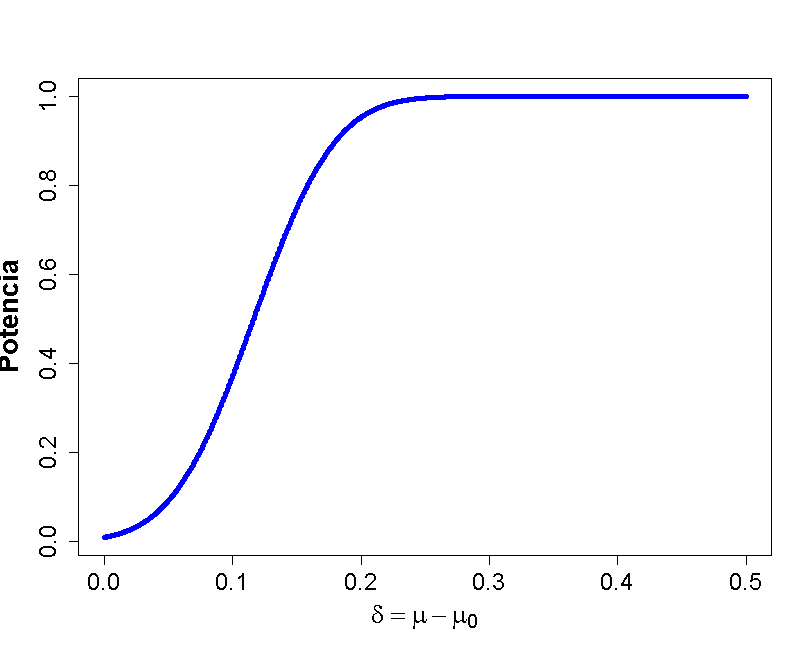
\includegraphics[width=10cm]{../fig/Cap07-CurvaPotencia.png}
\end{enColor}
\begin{bn}
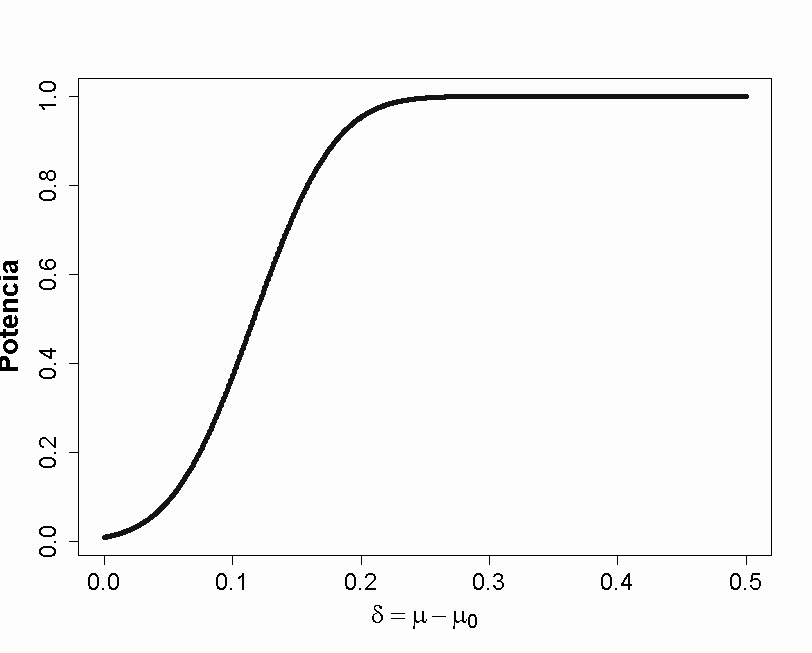
\includegraphics[width=10cm]{../fig/Cap07-CurvaPotencia-bn.png}
\end{bn}
\caption{Curva de potencia para un contraste de hipótesis con $H_0=\{\mu\leq \mu_0\}$, siendo $n=100$, $\alpha=0.01$ y $s=0.5$.}
\label{cap07:fig:CurvaPotencia}
\end{center}
\end{figure}



\section{Contrastes unilaterales y bilaterales.}
\label{cap07:sec:ContrastesUnilateralesBilaterales}

En las Secciones \ref{cap07:sec:LenguajeContrasteHipotesis} y \ref{cap07:sec:ContrasteHipotesisPasoaPaso} hemos presentado los elementos básicos del lenguaje del contraste de hipótesis, tomando siempre como referencia un ejemplo sobre la media, en el que la hipótesis alternativa era
    \[H_a=\{\mu>\mu_0\},\]
y la hipótesis nula era de la forma
    \[H_0=\{\mu\leq \mu_0\}.\]
Habíamos elegido esta hipótesis nula porque nuestra intención era mostrar que el tratamiento {\em aumentaba} el valor de la media. Y vimos (Ecuación \ref{cap07:ecu:pValorMediaZColaDerecha}, pág. \pageref{cap07:ecu:pValorMediaZColaDerecha}) que el p-valor es
\[
\mbox{p-valor}=P\left(Z > \dfrac{\bar X-\mu_0}{\dfrac{s}{\sqrt{n}}}\right)
\]
mientras que la región de rechazo de la hipótesis nula es de la forma (Ecuación \ref{cap07:ecu:RegionRechazoMediaZColaDerecha}, pág. \pageref{cap07:ecu:RegionRechazoMediaZColaDerecha}):
    \[R=\left\{\dfrac{\bar X-\mu_0}{\frac{s}{\sqrt{n}}}>z_{\alpha}\right\},\]
siendo $z_{\alpha}$ el valor crítico que, en la normal estándar  $N(0,1)$, deja una probabilidad $\alpha$ a su derecha. La región de rechazo tiene, en ese caso, el aspecto que se muestra en la Figura \ref{cap07:fig:RegionRechazoNormalColaDerecha}:

\begin{figure}[htbp]
\begin{center}
\begin{enColor}
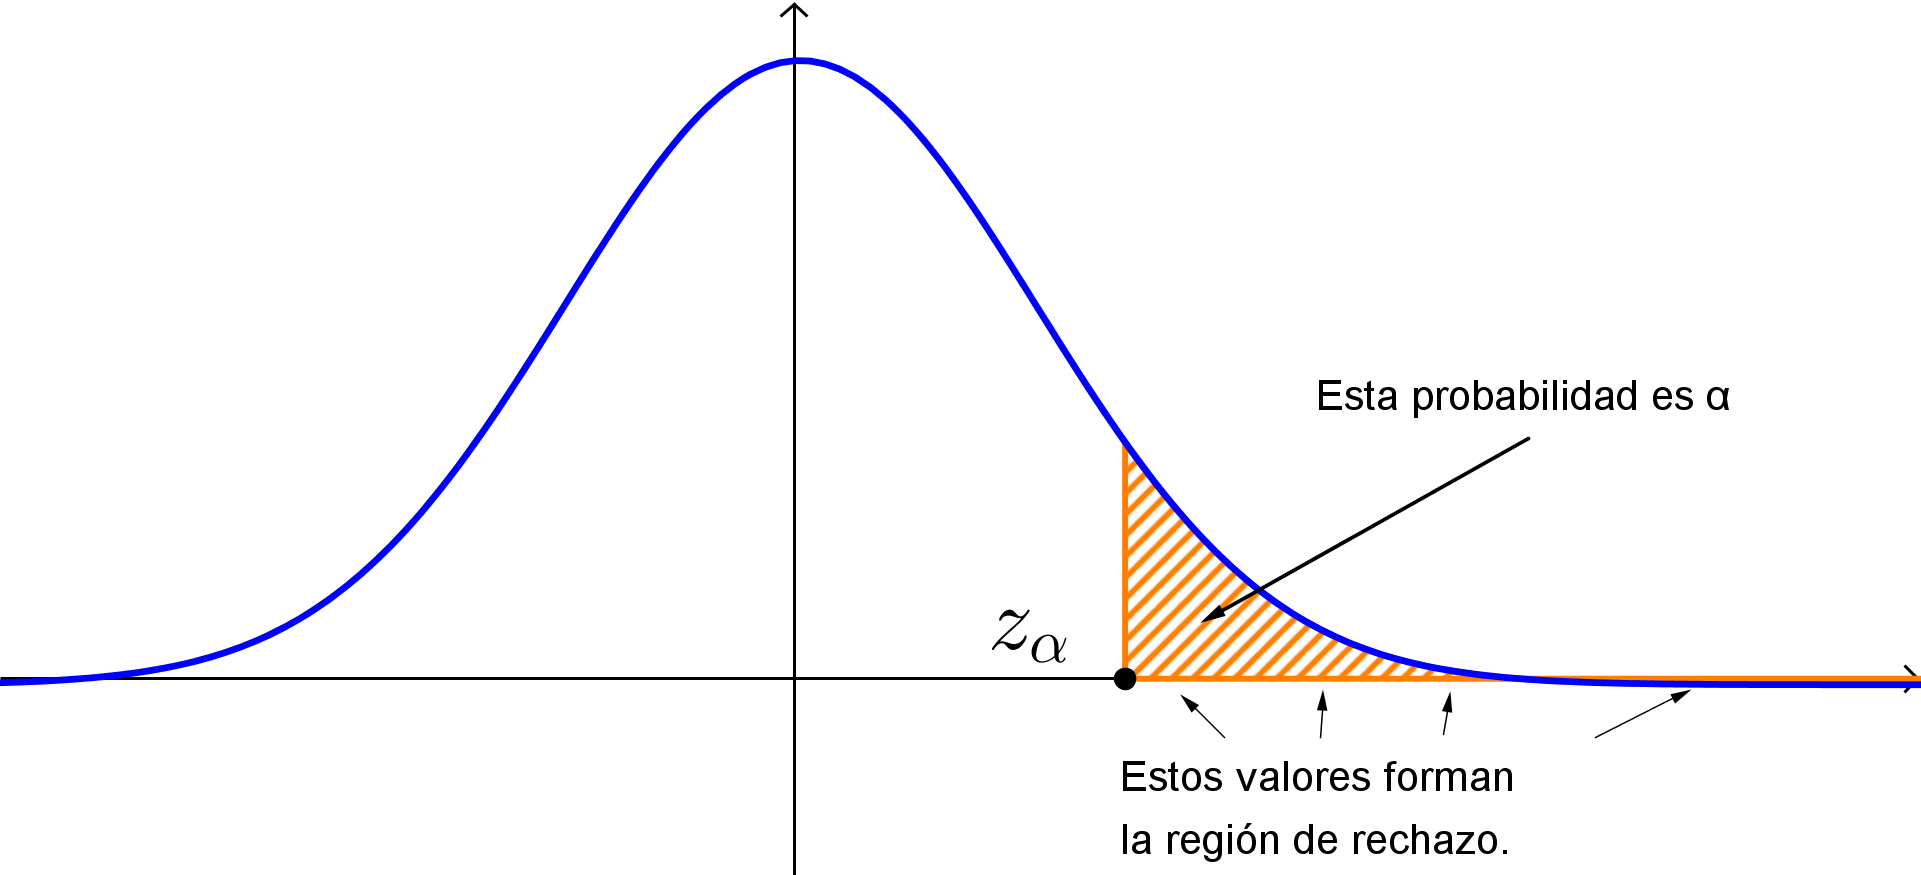
\includegraphics[width=13cm]{../fig/Cap07-RegionRechazoNormalColaDerecha.png}
\end{enColor}
\begin{bn}
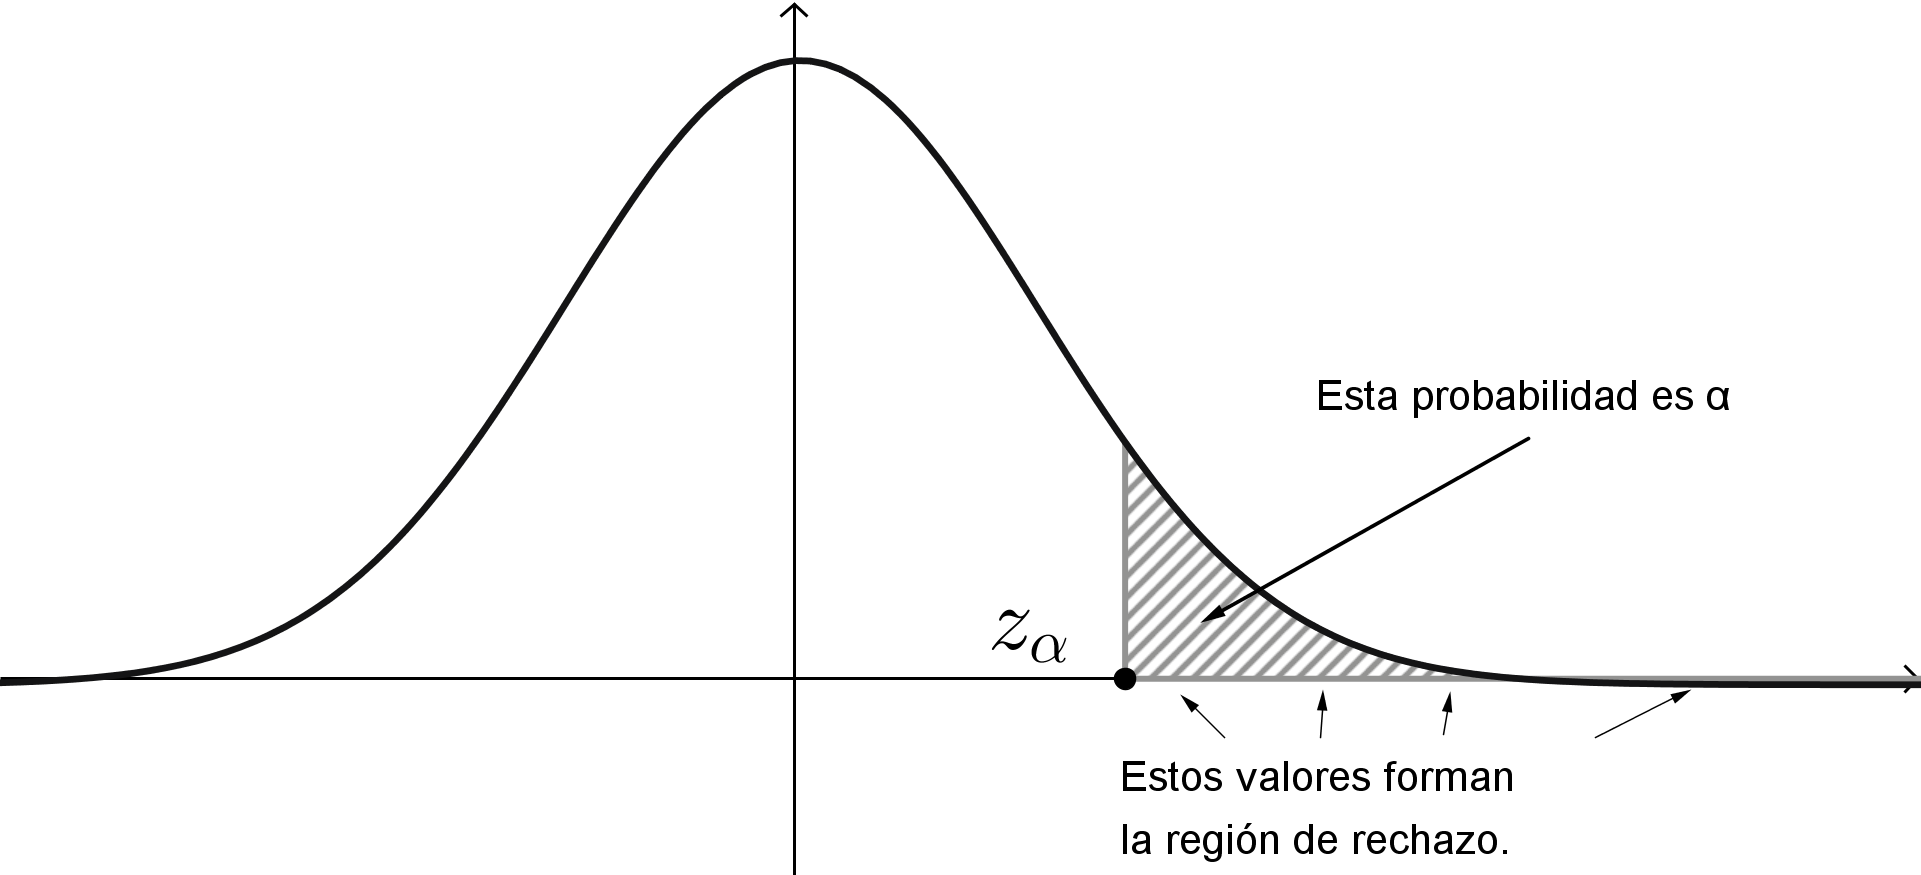
\includegraphics[width=13cm]{../fig/Cap07-RegionRechazoNormalColaDerecha-bn.png}
\end{bn}
\caption{Regi\'on de rechazo para $H_0=\{\mu\leq \mu_0\}$.}
\label{cap07:fig:RegionRechazoNormalColaDerecha}
\end{center}
\end{figure}

En otros problemas, sin embargo, puede que nuestra hipótesis sea distinta. Evidentemente, habrá ocasiones en que, lo que queremos, es analizar si el tratamiento ha disminuido la media. Y, en esos casos, la hipótesis nula será de la forma:
    \[H_0=\{\mu\geq \mu_0\},\quad \mbox{(mientras que  } H_a=\{\mu<\mu_0\}.\]
Ahora la región de rechazo de la hipótesis nula viene dada por
    \begin{equation}\label{cap07:ecu:RegionRechazoMediaZColaIzquierda}
        R=\left\{\dfrac{\bar X-\mu_0}{\frac{s}{\sqrt{n}}}<z_{1-\alpha}\right\},
    \end{equation}
siendo $z_{1-\alpha}$ el valor crítico que, en la normal estándar  $N(0,1)$, deja una probabilidad $\alpha$ a su izquierda. La región de rechazo es una cola izquierda de la distribución normal y tiene el aspecto que muestra la Figura \ref{cap07:fig:RegionRechazoNormalColaIzquierda}.

\begin{figure}[htbp]
\begin{center}
\begin{enColor}
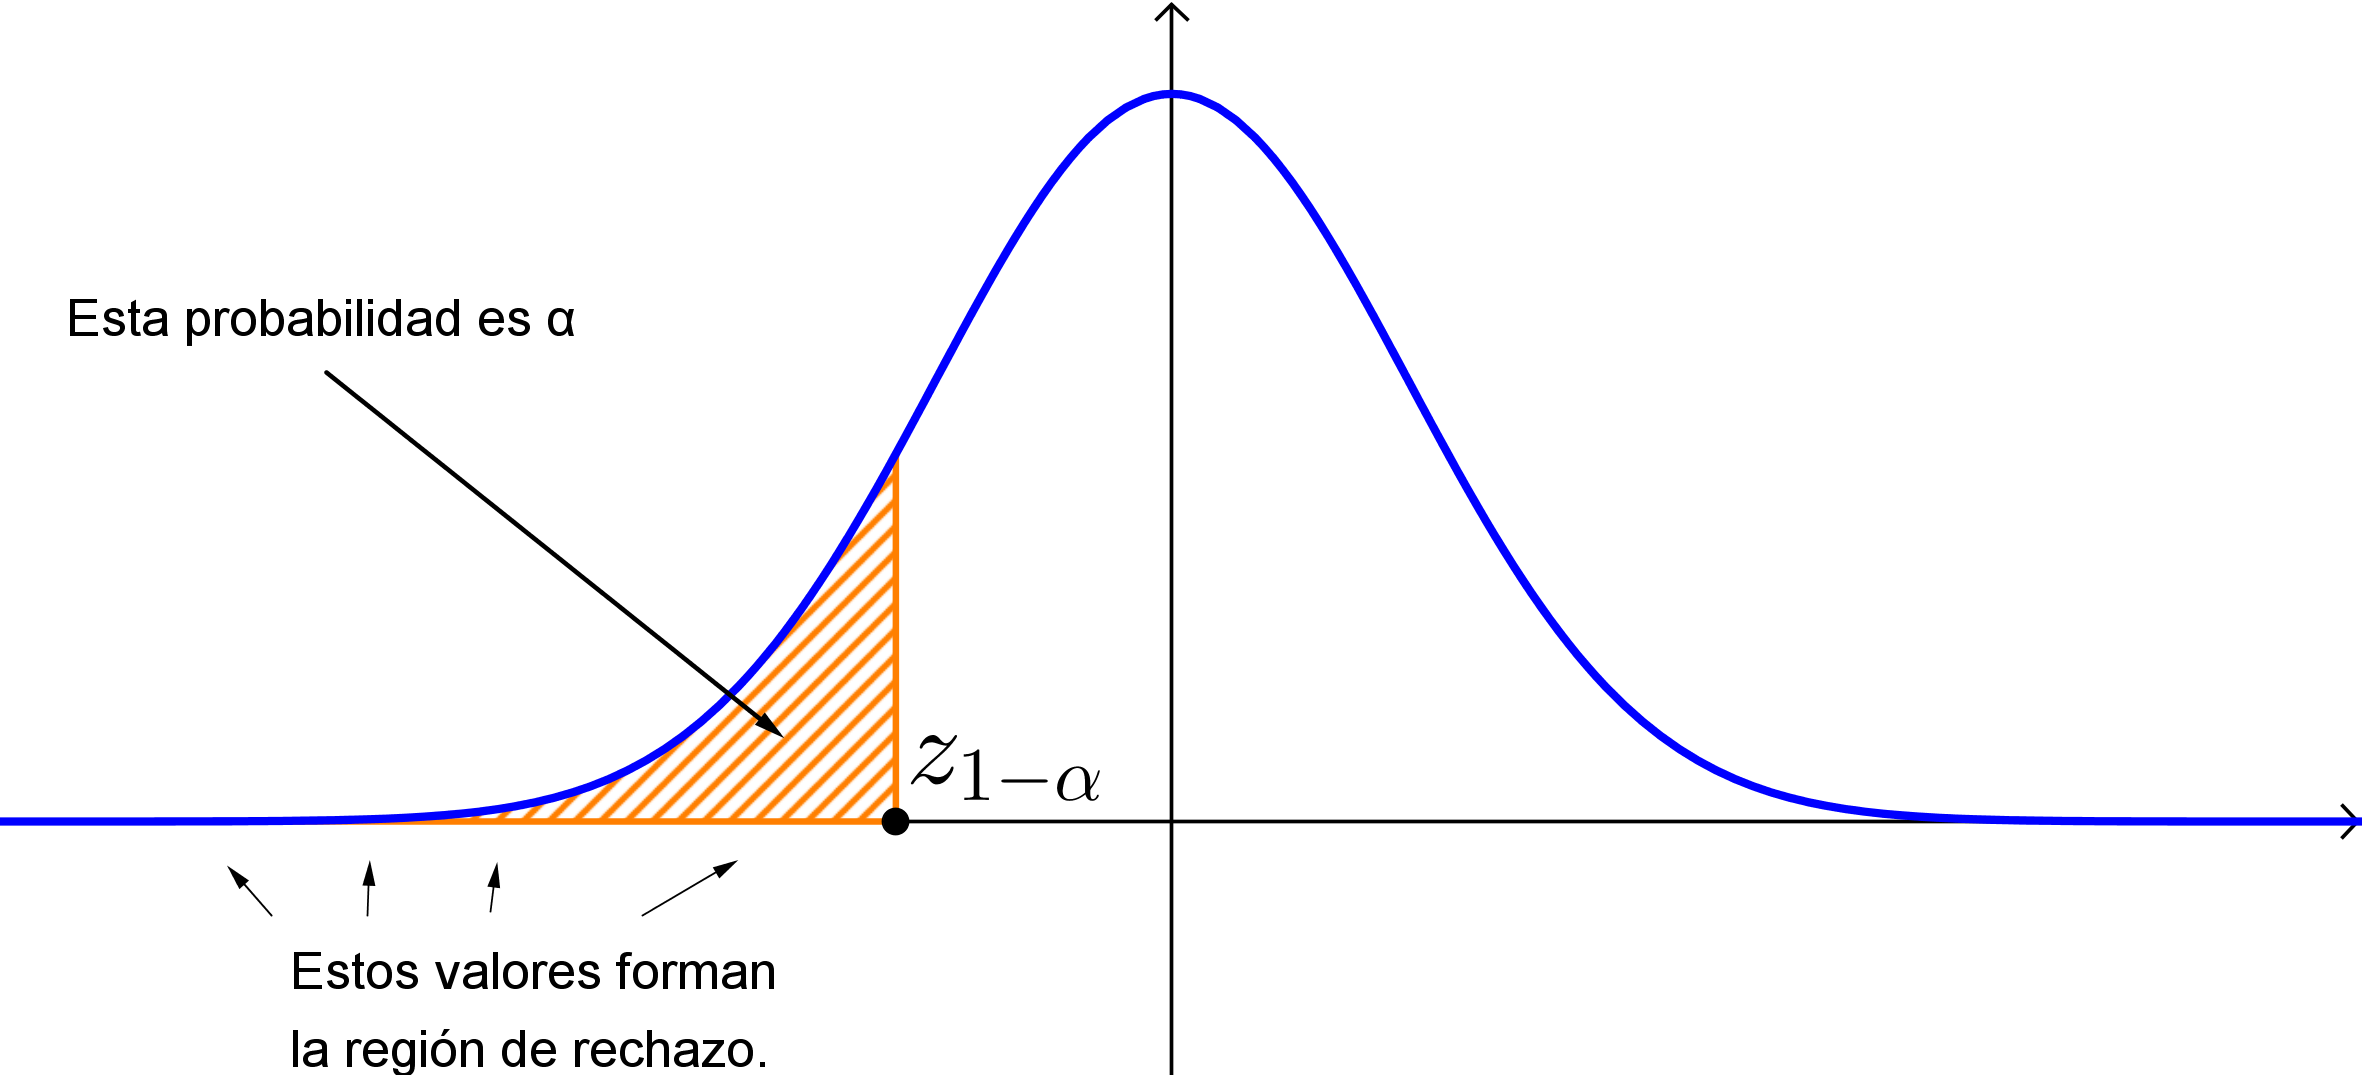
\includegraphics[width=13cm]{../fig/Cap07-RegionRechazoNormalColaIzquierda.png}
\end{enColor}
\begin{bn}
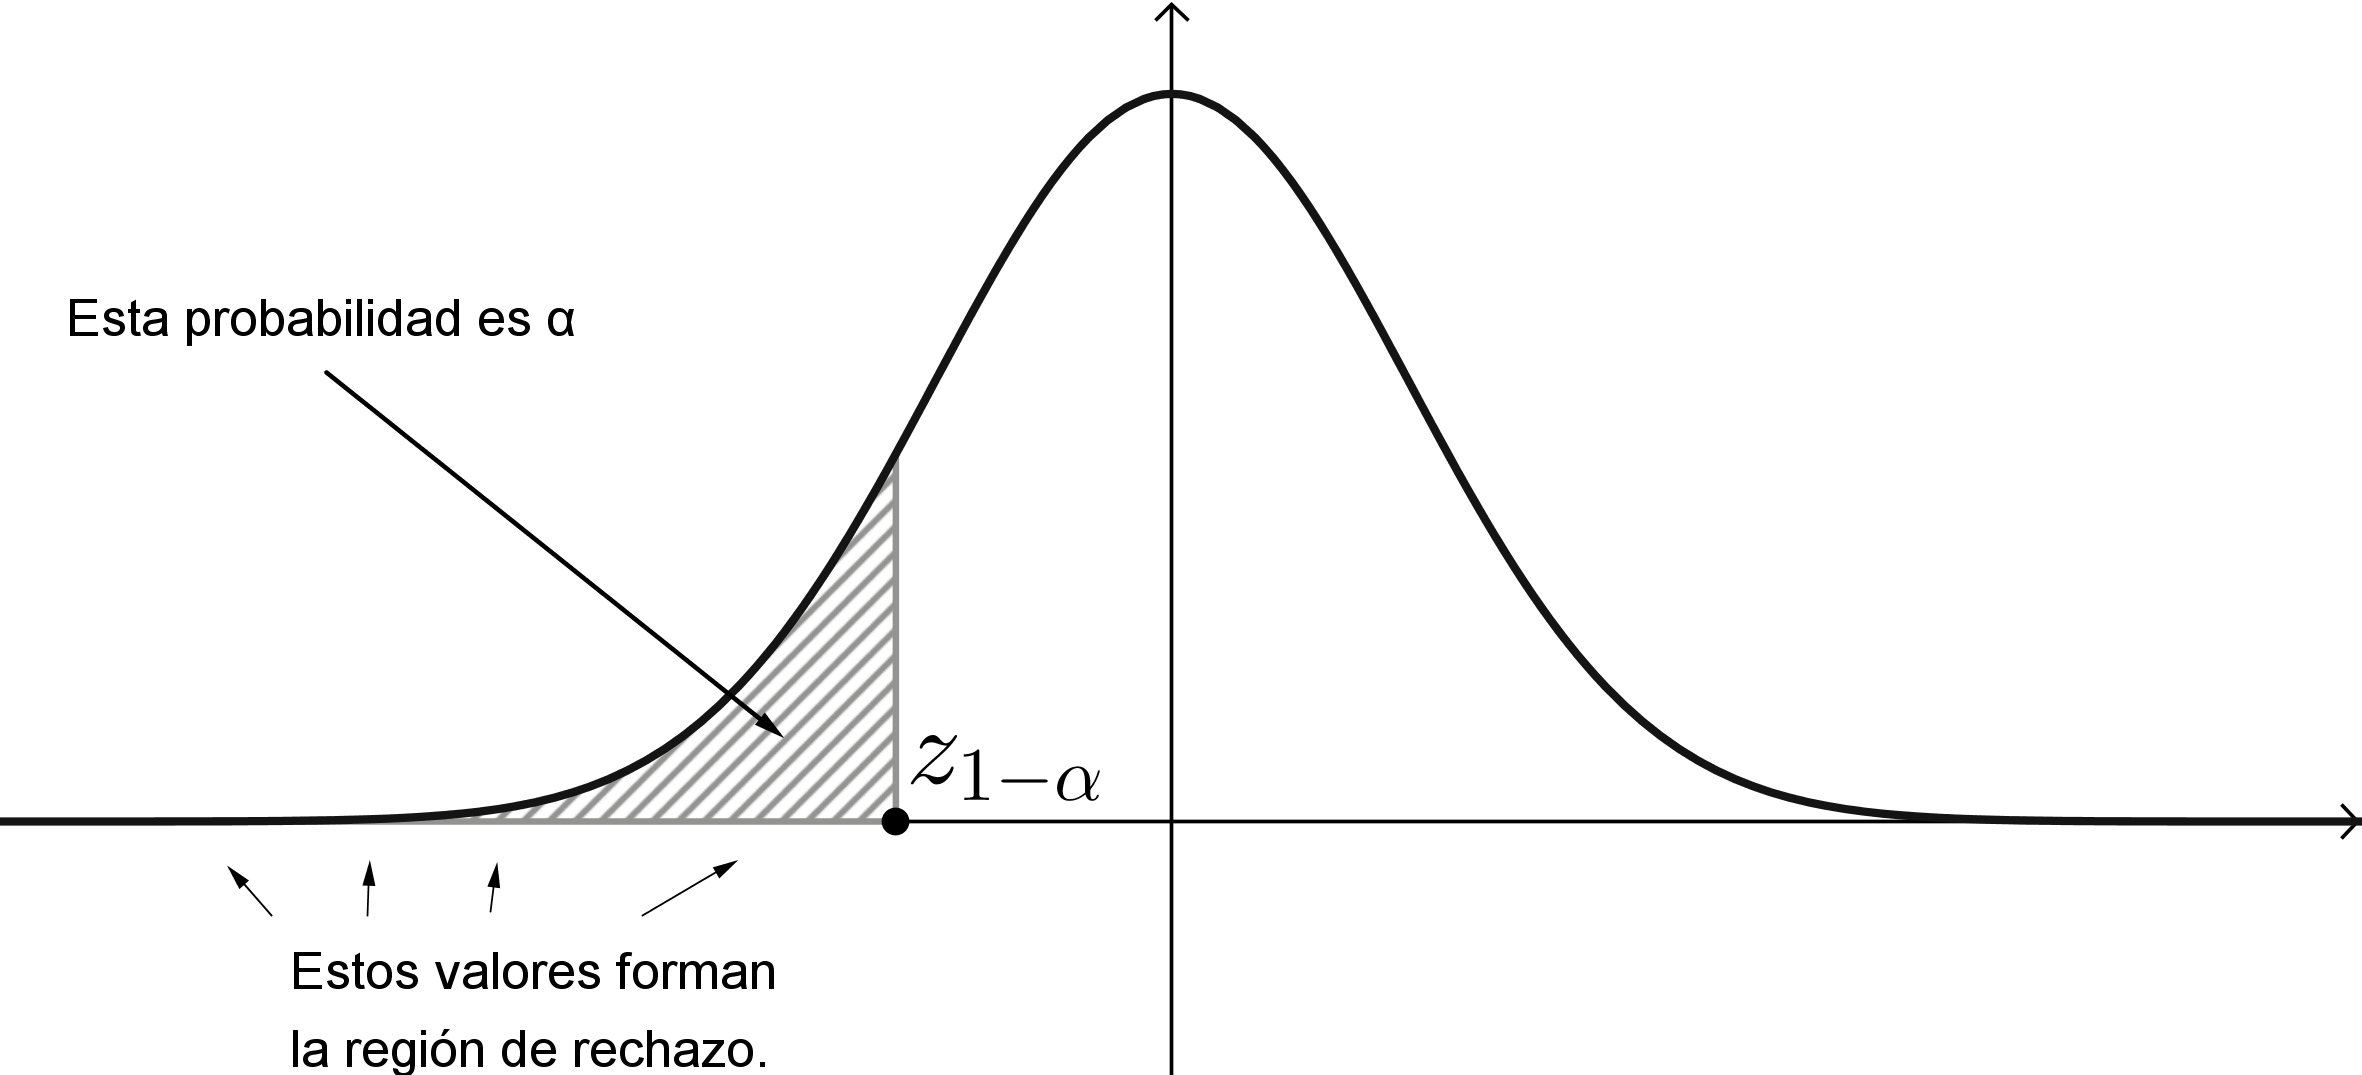
\includegraphics[width=13cm]{../fig/Cap07-RegionRechazoNormalColaIzquierda-bn.png}
\end{bn}
\caption{Regi\'on de rechazo para $H_0=\{\mu\geq \mu_0\}$.}
\label{cap07:fig:RegionRechazoNormalColaIzquierda}
\end{center}
\end{figure}

En un contraste como este, si se desea calcular el p-valor, debemos tener en cuenta que es igual a la probabilidad de la cola {\sf izquierda} que define el valor del estadístico. Es decir:
\begin{equation}\label{cap07:ecu:pValorMediaZColaIzquierda}
\mbox{p-valor}=
P\left(Z < \dfrac{\bar X-\mu_0}{\frac{s}{\sqrt{n}}}\right).
\end{equation}
%Es decir, que hacemos las mismas cuentas que en un contraste unilateral, pero multiplicamos la probabilidad resultante por 2, para tener en cuenta que la hipótesis alternativa se ve igualmente favorecida por valores alejados del origen, hacia cualquiera de los dos lados.
En ambos casos, la región de rechazo es una de las colas de la distribución (a derecha o a izquierda), y por eso los dos se denominan {\sf contrastes unilaterales}\index{contrastes unilaterales}.

Sin embargo, es posible que pensemos que el tratamiento tiene algún efecto, pero no sepamos (o no nos preocupe), a priori, si ese efecto va a hacer que la media sea más alta o más baja. En este caso, nuestra hipótesis alternativa es de la forma:
    \[H_a=\{\mu\neq\mu_0\}.\]
y la hipótesis nula es:
    \[H_0=\{\mu=\mu_0\}.\]
A diferencia de los dos casos anteriores, ahora la región de rechazo de la hipótesis nula la forman dos colas de la distribución. En concreto, la región de rechazo $R$ es de la forma:
    \begin{equation}\label{cap07:ecu:RegionRechazoMediaZBilateral}
        R=\left\{\left|\dfrac{\bar X-\mu_0}{\frac{s}{\sqrt{n}}}\right|>z_{\alpha/2}\right\},
    \end{equation}
siendo $z_{\alpha/2}$ el valor crítico que, en la normal estándar  $N(0,1)$, deja una probabilidad $1-\alpha/2$ a su izquierda (y por lo tanto, cada cola tiene probabilidad $\alpha/2$, como queremos).
En un caso como este hablamos de {\sf contraste bilateral}\index{contraste bilateral}. La región de rechazo tiene el aspecto que puede verse en la Figura \ref{cap07:fig:RegionRechazoNormalBilateral}.

\begin{figure}[htbp]
\begin{center}
\begin{enColor}
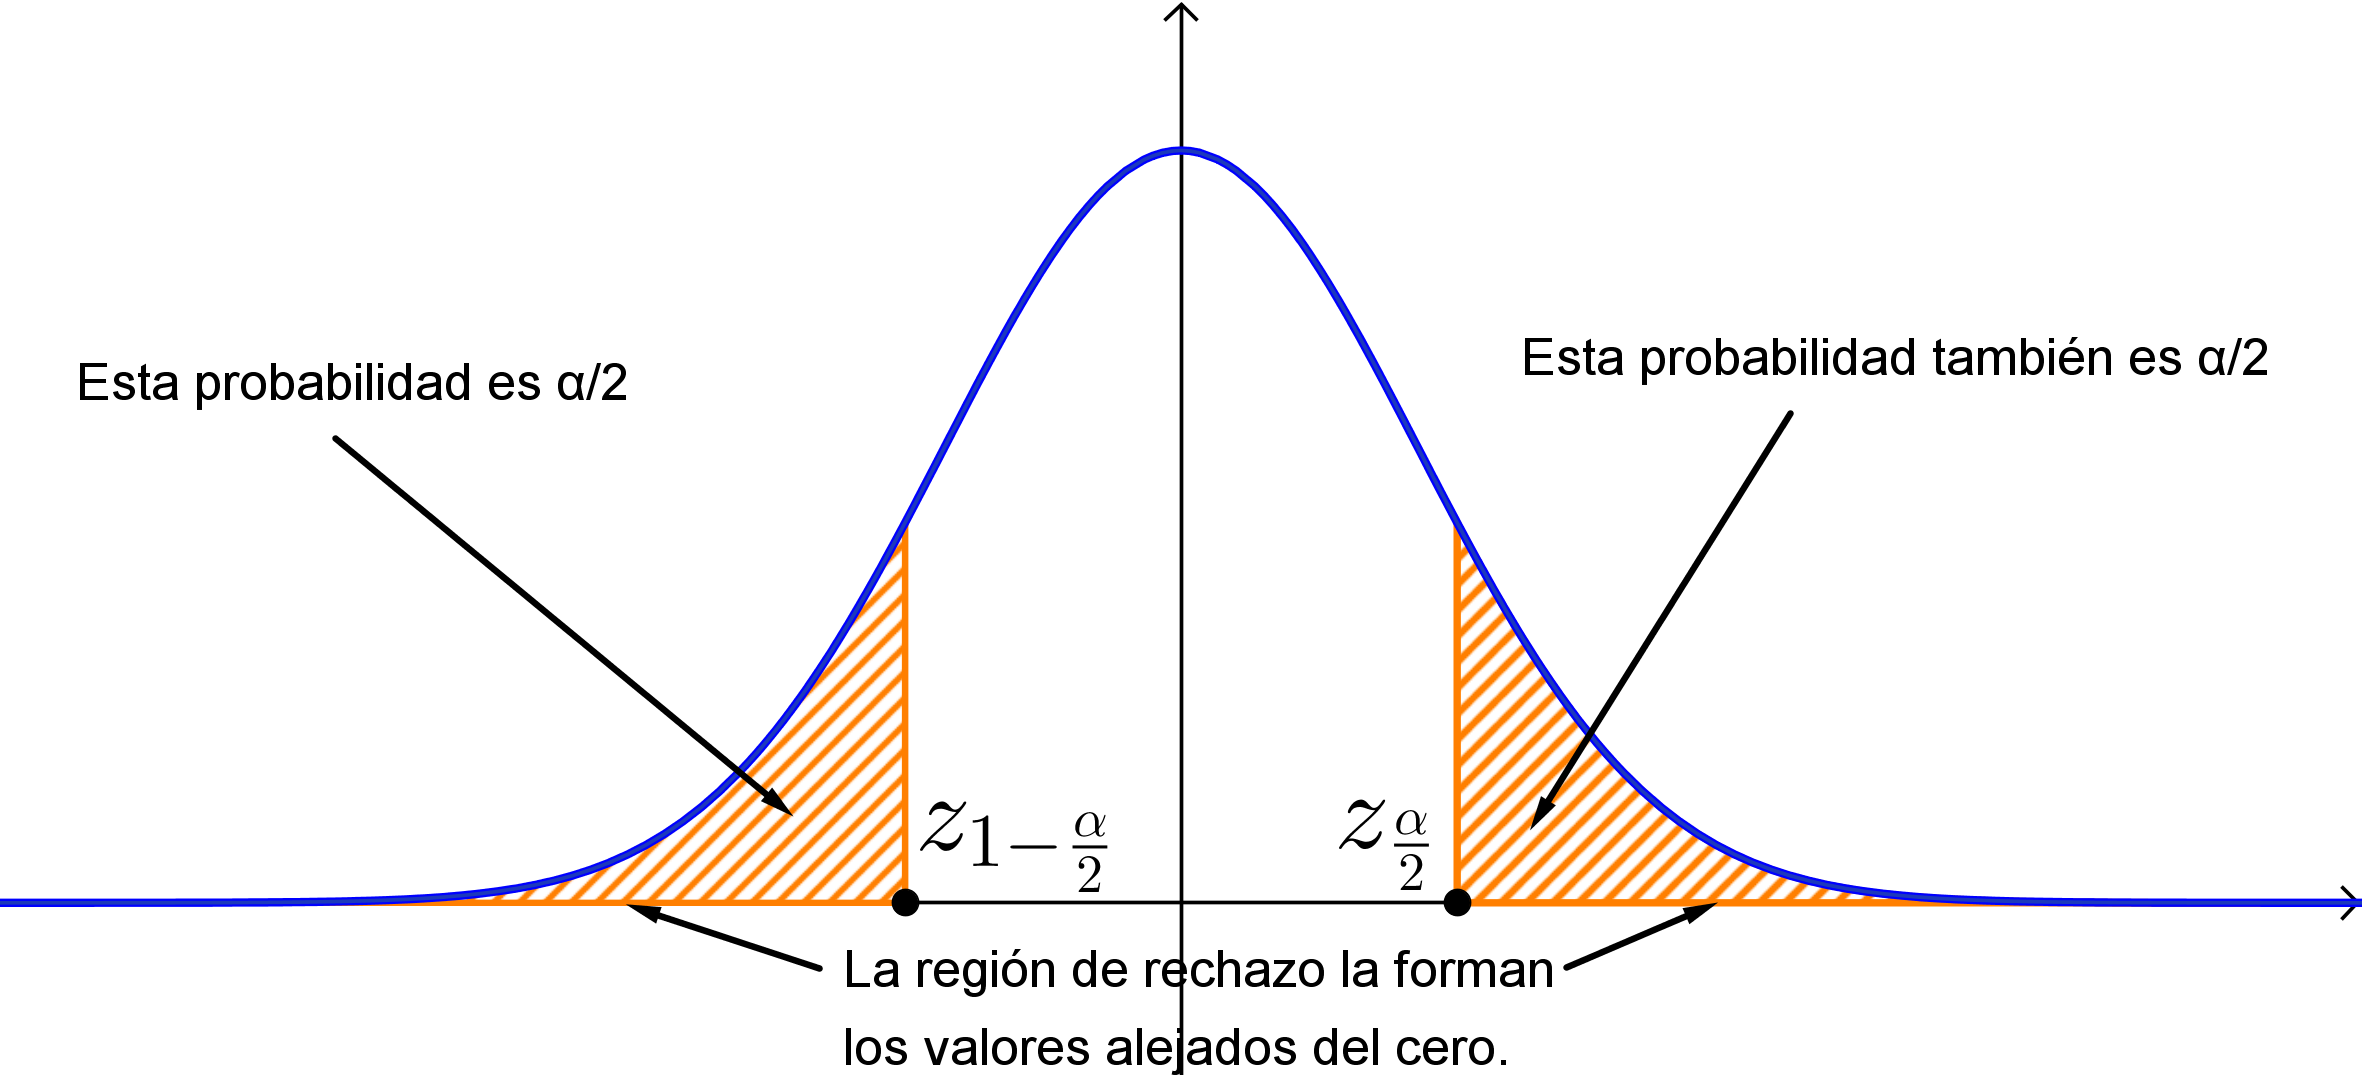
\includegraphics[width=13cm]{../fig/Cap07-RegionRechazoNormalBilateral.png}
\end{enColor}
\begin{bn}
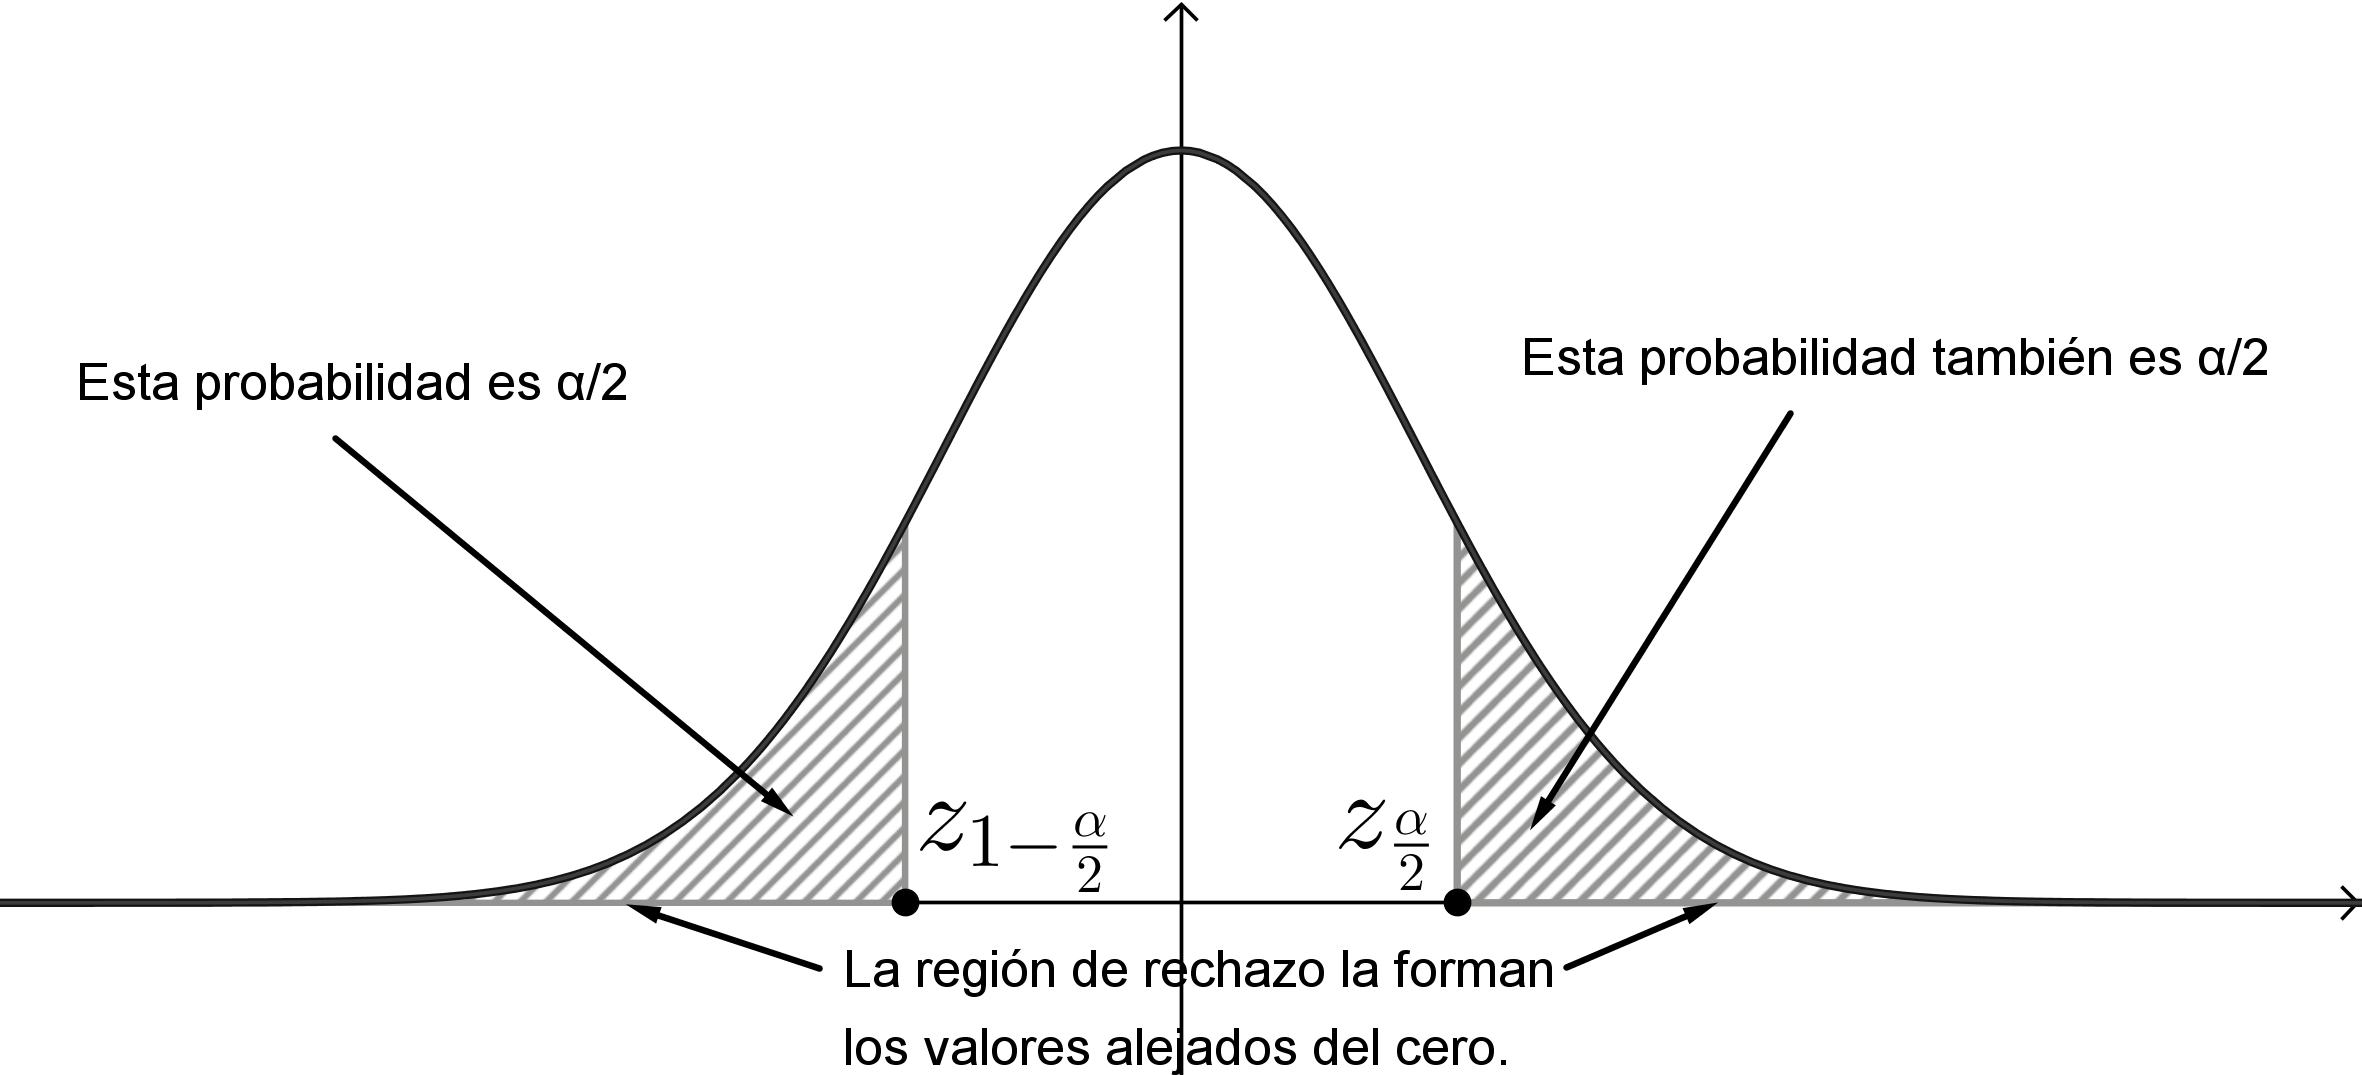
\includegraphics[width=13cm]{../fig/Cap07-RegionRechazoNormalBilateral-bn.png}
\end{bn}
\caption{Regi\'on de rechazo para $H_0=\{\mu = \mu_0\}$.}
\label{cap07:fig:RegionRechazoNormalBilateral}
\end{center}
\end{figure}

El p-valor, en el caso bilateral, es especial. Puesto que debemos tener en cuenta que hay dos colas, se calcula mediante:
\begin{equation}
\label{cap07:ecu:pValorMediaZBilateral}
\mbox{p-valor}=\colorbox{lightgrey}{\large\bf 2}\cdot P\left(Z > \dfrac{ \colorbox{lightgrey}{$|\bar X-\mu_0|$}}{\dfrac{s}{\sqrt{n}}}\right)
\end{equation}
El valor absoluto aquí es {\bf muy importante}. Porque si la muestra produce $\bar X<\mu$, tendremos $\bar X-\mu<0$. Si no tomamos el valor absoluto, la probabilidad que aparece en  \ref{cap07:ecu:pValorMediaZBilateral} será mayor que $1/2$, y terminaremos con un p-valor mayor que uno, lo cual no tiene sentido. {!`}De nuevo, piensa siempre sobre una figura!

\paragraph{Contraste bilateral e intervalo de confianza.}
\label{cap07:lugar:ContrasteBilateralIntervaloConfianza}
Este último caso es el que más recuerda a los intervalos de confianza, porque los valores críticos de $Z$ que se usan son los mismos. De hecho, si quieres entretenerte en pensarlo, un valor $\mu_0$ que esté fuera del intervalo de confianza (al nivel de confianza $nc=1-\alpha$), produce siempre un valor del estadístico situado en la región de rechazo (al nivel de significación $ns=1-\alpha$), y viceversa. Pero si esto te resulta muy confuso, por el momento no te preocupes, la relación entre contrastes de hipótesis e intervalos de confianza irá quedando más clara en posteriores capítulos. Por ejemplo, volveremos sobre esto en la Sección \ref{cap09:subsec:IntervalosDeConfianzaVsContrastes01}.\\

Antes de cerrar este apartado, queremos incluir un ejemplo que trata de ilustrar uno de los errores más comunes que cometen quienes se inician en el tema de los contrastes de hipótesis, para prevenir al lector.
\begin{ejemplo}\label{cap07:ejem:ErrorTipicoContrastesHipotesis}
Supongamos que, en el Ejemplo \ref{cap07:ejem:CangurosDepresivos01}, de los canguros depresivos saltarines, y con hipótesis nula
    \[H_0=\{\mu\leq \mu_0=2.5\},\]
hubiéramos obtenido una muestra con estos valores:
    \[n=100,\quad \bar X=2.35,\quad s=0.5\]
Siguiendo los pasos que hemos descrito, calculamos el valor del estadístico adecuado, que es
    \[
    Z=\dfrac{\bar X-\mu_0}{\dfrac{s}{\sqrt{n}}}=\dfrac{2.35-2.5}{\dfrac{0.5}{\sqrt{100}}}=
    \dfrac{-0.15}{\dfrac{0.5}{10}}=-3.
    \]
Puesto que el valor del Estadístico es negativo, la Figura \ref{cap07:fig:RegionRechazoNormalColaIzquierda} se nos aparece y nos lleva a calcular el p-valor usando la cola izquierda de la distribución.  Es decir, que calculamos (usando el ordenador)
\[P\left(Z < -3\right)\approx 0.001350.\]
Y con ese p-valor tan pequeño, rechazamos de plano $H_0$, sin la menor duda.

{!`}Esto está mal, mal, mal! El p-valor debería hacerse con la cola derecha (enseguida daremos las razones), calculando:
\[P\left(Z > -3\right)\approx 1-0.001350=0.99875.\]
Y el problema es que, seguramente, la inexperiencia, unida al hecho de que normalmente buscamos p-valores pequeños, hace desconfiar de este valor, que es el correcto.

Vamos despacio, para intentar que el lector entienda lo que sucede. Para empezar: debemos usar la cola derecha, porque la hipótesis nula es $H_0=\{\mu\leq \mu_0\}$, mientras que la Figura \ref{cap07:fig:RegionRechazoNormalColaIzquierda} se refiere al caso $H_0=\{\mu\geq \mu_0\}$. ¿Qué es lo que sucede en este ejemplo, para que las cosas sean así de raras? Pues lo que sucede es que la muestra ha producido una altura media $\bar X=2.35$, y nosotros (en realidad $H_a$) pretendemos usar esto para demostrar que $\mu > 2.5$. {!`}Pero cómo va a ser mayor, si los datos de la muestra son menores! En todo caso, volviendo al tema del ejemplo, esta muestra serviría para probar que {\em Pildorín Complex} ha hundido a los pobres canguros en una depresión aún más profunda.
\qed
\end{ejemplo}
Este ejemplo pretende poner en guardia al lector sobre el hecho de que, aunque el contraste siempre puede realizarse, y el p-valor siempre puede calcularse, si los valores de la muestra contradicen flagrantemente a la hipótesis alternativa, sólo podemos esperar un p-valor muy alto, y desde luego, debemos abandonar cualquier idea de rechazar $H_0$. Y además, siempre, siempre, debemos pensar en qué tipo de contraste estamos haciendo, y preguntarnos si queremos ver una Figura como \ref{cap07:fig:RegionRechazoNormalColaDerecha} o como \ref{cap07:fig:RegionRechazoNormalColaIzquierda}, antes de sustituir los valores muestrales en el estadístico. De esa forma nos será más difícil equivocar una cola izquierda por una derecha y viceversa.


\section{Contraste de hipótesis para la media de poblaciones normales con muestras pequeñas.}
\label{cap07:sec:contrasteHipotesisMediaMuestrasPequennas}

Al igual que sucedía con los intervalos de confianza, si el tamaño de la muestra es pequeño (recordemos, $n<30$), debemos reemplazar la normal estándar $Z$ por la $t$ de Student. Aparte de este cambio, los contrastes de hipótesis son muy similares, utilizando los valores críticos $t_{k;p}$ de la distribución $t$ de Student, en lugar de los $z_p$. Se obtienen estos resultados:
\begin{enumerate}
    \item Hipótesis alternativa: $H_a=\{\mu>\mu_0\}$, hipótesis nula: $H_0=\{\mu\leq \mu_0\}$.\\[3mm]
            Región de rechazo $R$ de la forma:
            \[R=\left\{\dfrac{\bar X-\mu_0}{\frac{s}{\sqrt{n}}}>t_{k;\alpha}\right\},\]
            siendo $t_{k;\alpha}$ el valor crítico para la distribución $t$ de Student con $k=n-1$ grados de libertad, que deja una probabilidad $\alpha$ a su derecha.

            Cálculo del p-valor:
            \begin{equation}\label{cap07:ecu:pValorMediaStudentColaIzquierda}
            \mbox{p-valor}=
            P\left(T_k > \dfrac{\bar X-\mu_0}{\frac{s}{\sqrt{n}}}\right).
            \end{equation}


    \item Hipótesis alternativa: $H_a=\{\mu<\mu_0\}$, hipótesis nula: $H_0=\{\mu\geq \mu_0\}$.\\[3mm]
            Región de rechazo $R$ de la forma:
            \[R=\left\{\dfrac{\bar X-\mu_0}{\frac{s}{\sqrt{n}}}<t_{k;1-\alpha}\right\},\]
            siendo $t_{k;1-\alpha}=-t_{k;\alpha}$ el valor crítico para la distribución $t$ de Student con $k=n-1$ grados de libertad, que deja una probabilidad $\alpha$ a su izquierda.

            Cálculo del p-valor:
            \begin{equation}\label{cap07:ecu:pValorMediaStudentColaIzquierda}
            \mbox{p-valor}=
            P\left(T_k < \dfrac{\bar X-\mu_0}{\frac{s}{\sqrt{n}}}\right).
            \end{equation}


    \item Hipótesis alternativa: $H_a=\{\mu\neq\mu_0\}$, hipótesis nula: $H_0=\{\mu=\mu_0\}$.\\[3mm]
            Región de rechazo $R$ de la forma:
        \[R=\left\{\left|\dfrac{\bar X-\mu_0}{\frac{s}{\sqrt{n}}}\right|>t_{k;\alpha/2}\right\},\]
        siendo $t_{k;\alpha/2}$ el valor crítico para la distribución $t$ de Student con $k=n-1$ grados de libertad, que deja una probabilidad $\alpha/2$ a su derecha (y por lo tanto, cada cola tiene probabilidad $\alpha/2$).

        Cálculo del p-valor:
        \begin{equation}\label{cap07:ecu:pValorMediaZBilateral}
        \mbox{p-valor}= 2\cdot P\left(T_k > \dfrac{ \colorbox{white}{$|\bar X-\mu_0|$}}{\dfrac{s}{\sqrt{n}}}\right)
        \end{equation}


    \end{enumerate}

\noindent Veamos un ejemplo.
\begin{ejemplo}\label{cap07:ejem:ContrasteMediaMuestrasPequennas}
Un fabricante de teléfonos móviles afirma que la batería de sus teléfonos tiene una duración de 36 horas. Para comprobarlo se dispone de una muestra de 10 teléfonos, y se comprueba que tardan en descargarse, en promedio, 34.5 horas, con una cuasidesviación muestral de 3.6 horas. Contrastar la afirmación del fabricante.

En un ejemplo como este, lo primero que debemos hacer es dejar claro cuál es la hipótesis alternativa $H_a$ que queremos contrastar (la hipótesis nula será entonces evidente). Y en algunos casos, hay dos formas de interpretar el enunciado. Por un lado, pensemos en una asociación de consumidores, preocupada porque les han llegado quejas de que las baterías de estos teléfonos duran menos de lo que dice su publicidad. Para esa asociación, la hipótesis alternativa que hay que contrastar es
    \[H_a={\mu<\mu_0},\]
siendo $\mu_0=36$ horas, es decir, la duración que anuncia el fabricante. Es decir que la asociación escribe como hipótesis alternativa su sospecha de que la media real $\mu$ es menor que $\mu_0=36$ horas. La hipótesis nula, naturalmente, es en este caso
    \[H_0={\mu\geq \mu_0}.\]
Por otro lado, el fabricante de estos teléfonos sabe que el proceso de fabricación de las baterías es costoso, y que aumentar en un par de horas su duración puede suponer un aumento intolerable de ese coste. Naturalmente, tampoco quiere incurrir en publicidad engañosa y enfrentarse a una posible sanción y a la pérdida de prestigio aparejada. Así que, para el fabricante, la pregunta es si es los datos son compatibles con su afirmación de que la batería dura 36 horas. Dicho de otra manera, el fabricante se pregunta ``¿voy a tener problemas si digo que la duración media es de 36 horas?'' Al mismo tiempo, tampoco le interesa que la duración sea mucho mayor, porque si lo fuera, sería más rentable abaratar la fabricación de las baterías, y a la vez mantener esa publicidad. Para el fabricante, entonces, la hipótesis alternativa a contrastar es:
    \[H_a={\mu\neq \mu_0},\]
donde, como antes, $\mu_0=36$ horas. La hipótesis nula, en este caso es
    \[H_0={\mu = \mu_0}.\]
Como puede verse, no hay un contraste ``correcto'', sino respuestas distintas a preguntas distintas. A menudo, al abordar un contraste y decidir cuáles son las hipótesis, es conveniente pensar cuál es el ``personaje'' de la historia que hace la pregunta, porque eso nos ayuda a aclarar precisamente eso: qué pregunta estamos haciendo.


Para empezar, supongamos que la pregunta la hace la asociación de consumidores. Entonces la hipótesis nula es (caso 2)
    \[H_0={\mu\geq \mu_0}.\]
Calculamos el estadístico adecuado para este contraste:
     \[\dfrac{\bar X-\mu_0}{\frac{s}{\sqrt{n}}}=\dfrac{34.5-36}{\frac{3.5}{\sqrt{10}}}\approx -2.196\]
Y con eso calculamos el p-valor mediante
\[\mbox{p-valor}=
            P\left(T_k < \dfrac{\bar X-\mu_0}{\frac{s}{\sqrt{n}}}\right),\]
%(en R usaríamos {\tt pt(Estadistico,df=k)}, porque es una cola izquierda)
que es, aproximadamente
\[\mbox{p-valor}\approx 0.028\]
Es decir, que puesto que el p-valor es menor que $0.05$, rechazamos la hipótesis nula al 95\%.

¿Qué sucede cuando es el fabricante el que hace las cuentas? Para el fabricante, el valor del estadístico es el mismo (en valor absoluto), pero el cálculo del p-valor se hace usando:
\[        \mbox{p-valor}= 2\cdot P\left(T_k > \dfrac{ \colorbox{white}{$|\bar X-\mu_0|$}}{\dfrac{s}{\sqrt{n}}}\right)
\]
Así que se obtiene:
\[\mbox{p-valor}\approx 0.056\]
y por lo tanto, aunque por muy poco, el fabricante no rechaza la hipótesis nula, y se da por satisfecho.

¿Y entonces? Bueno, la decisión seguramente no estará en manos de ninguno de ellos, sino de las autoridades o tribunales de consumo. Así que si quieren saber a que atenerse, tanto el fabricante como los consumidores deben averiguar cuál es la pregunta relevante para esas instancias.
\qed
\end{ejemplo}


\section{Contraste de hipótesis para $\sigma^2$ en poblaciones normales.}
\label{cap07:sec:contrasteHipotesisSigma2}

Al igual que hicimos en el Capítulo \ref{cap:IntervalosConfianza}, vamos a completar el estudio de las poblaciones normales, extendiendo el lenguaje del contraste de hipótesis a los problema relacionados con la varianza $\sigma^2$. No hace falta desarrollar ningún recurso teórico nuevo, porque todo lo que necesitamos está contenido en la Ecuación \ref{cap06:ecu:EstadisticoParaSigmaCuadrado} (pág. \pageref{cap06:ecu:EstadisticoParaSigmaCuadrado}), en la que obtuvimos el estadístico adecuado para entender la distribución muestral de $\sigma^2$, que era:
\[(n-1)\dfrac{s^2}{\sigma^2}\sim\chi^2_k,\mbox{ con }k=n-1.\]
Una vez que disponemos de esta información, el esquema básico de los contrastes es el mismo que hemos usado con la media. Se obtienen los resultados que aparecen a continuación. En todos los casos se supone que se trata de una población normal, de tipo $N(\mu,\sigma)$), y se utilizan muestras aleatorias de tamaño $n$. El valor del estadístico:
       \[Y=(n-1)\dfrac{s^2}{\sigma_0^2},\]
se ha calculado sobre la muestra, y usando el valor $\sigma_0$ que aparece en la correspondiente hipótesis nula.
\begin{enumerate}
       \item[(a)] Hipótesis nula: $H_0=\{\sigma^2\leq \sigma^2_0\}$. Región de rechazo: \[\sigma_0^2<\dfrac{(n-1)s^2}{\chi^2_{k,\alpha}}.\]
           p-valor$=P\left(\chi^2_k> Y\right),$ (cola derecha del estadístico)
       \item[(b)] Hipótesis nula: $H_0=\{\sigma^2\geq \sigma^2_0\}$. Región de rechazo: \[\sigma_0^2>\dfrac{(n-1)s^2}{\chi^2_{k,1-\alpha}}.\]
           p-valor$=P\left(\chi^2_k< Y\right),$ (cola izquierda del estadístico).
       \item[(c)] Hipótesis nula: $H_0=\{\sigma^2=\sigma^2_0\}$. Región de rechazo: \[(n-1)\dfrac{s^2}{\sigma_0^2}\mbox{ no pertenece al intervalo:}
            \left(\chi^2_{k,1-\alpha/2},\chi^2_{k,\alpha/2}\right).\]
           p-valor$=2\cdot P\left(\chi^2_k> Y\right)$. Esta fórmula es correcta si el estadístico es $>k$ (es decir, cuando $s>\sigma_0$); si es $<k$ (cuando $s<\sigma_0$), debemos usar la cola izda. y multiplicar por dos. Esta situación es análoga a la discusión que hicimos para la Ecuación \ref{cap07:ecu:pValorMediaZBilateral}. Si no se presta atención al valor de la muestra, podemos terminar con un p-valor mayor que uno.
\end{enumerate}
Veamos un ejemplo.

\begin{ejemplo}\label{cap07:ejem:ContrasteVarianzaLatasConserva}
Para que un lote de tornillos sea aceptable, la desviación típica de sus longitudes no debe superar los 0.2mm. Para examinar un lote de 5000 tornillos, hemos tomado una muestra aleatoria de 15 tornillos, y hemos obtenido una cuasidesviación típica igual a $0.24$mm. ¿Estamos justificados para rechazar la hipótesis nula $H_0=\{\sigma\leq \sigma_0\}$ (donde $\sigma_0=0.2$)?

Para saberlo calculamos el estadístico:
\[Y=(n-1)\dfrac{s^2}{\sigma_0^2}= 14\dfrac{0.24^2}{0.2^2}\approx 20.16,\]
y obtenemos el p-valor (como de costumbre, usando el ordenador),  mediante
\[\mbox{p-valor}=P\left(\chi^2_k> Y\right)\approx 0.13,\]
así que no rechazaremos $H_0$.
\qed
\end{ejemplo}
